\chapter{Hasil dan Diskusi}

Bab ini menyajikan hasil implementasi \textit{pipeline} pada dua studi kasus: 
kode PHP milik FT UGM (Dashboard TCK) dan kode PHP milik DTI UGM (Sistem CBT), 
beserta analisis perbandingan keduanya. Pembahasan studi kasus pertama mencakup: hasil konversi Rector, 
hasil pemindaian keamanan Semgrep sebelum dan sesudah konversi, 
hasil validasi PHPStan, status kepatuhan ISO/IEC 27001:2022, 
analisis dependensi \textit{composer}, hasil komparasi lima model 
LLM dengan \textit{prompt} identik (Kondisi A), hasil komparasi 
dengan \textit{prompt} yang dioptimasi per model (Kondisi B), 
optimasi parameter Qwen2.5-Coder (Kondisi C), serta diskusi dan 
keterbatasan penelitian. Bagian penutup menyajikan perbandingan hasil kedua 
studi kasus secara menyeluruh.

% ============================================================
\section{Hasil Konversi Rector}
% ============================================================

Rector dijalankan terhadap 245 \textit{file} PHP dari dataset FT UGM dengan target versi PHP 8.3. Dari 245 \textit{file} tersebut, 239 \textit{file} berhasil dikonversi, 4 \textit{file} dilewati (\textit{skipped}), dan 2 \textit{file} gagal diproses. Tingkat konversi keseluruhan ($CR = 97{,}6\%$), sebagaimana ditunjukkan pada Gambar \ref{fig:rector-conversion}.

\begin{figure}[h]
    \centering
    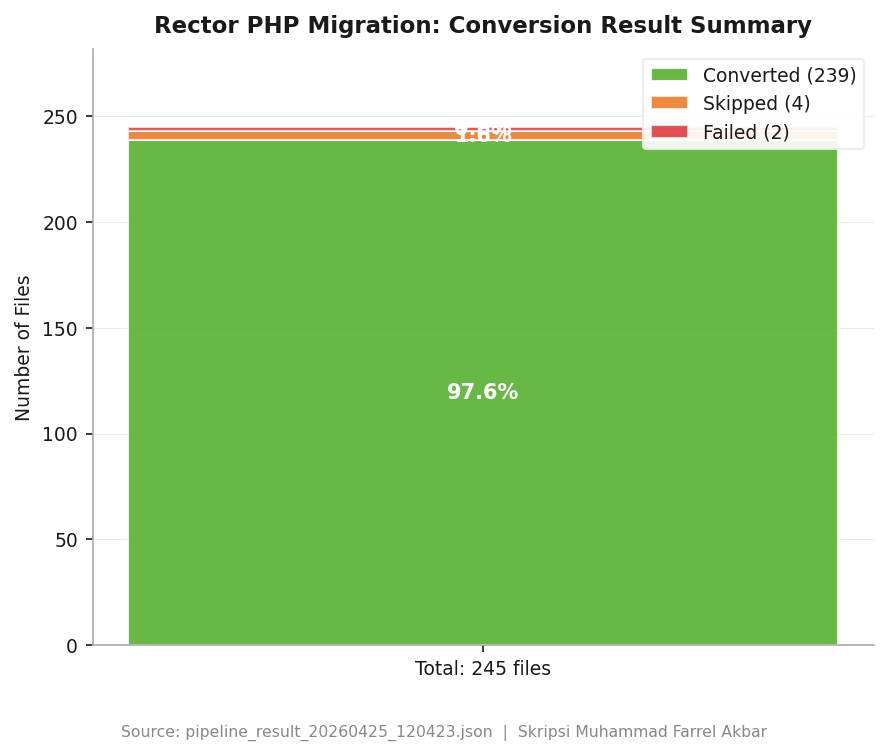
\includegraphics[width=0.8\textwidth]{contents/chapter-4/pipeline_chart_20260425_182849_3_rector_conversion.png}
    \caption{Ringkasan hasil konversi Rector terhadap 245 \textit{file} PHP dataset FT UGM}
    \label{fig:rector-conversion}
\end{figure}
\newpage
Karena dataset mengandung campuran kode PHP 5.x dan PHP 7.x, Rector menerapkan rantai \textit{ruleset} kumulatif dari \texttt{UP\_TO\_PHP\_53} hingga \texttt{UP\_TO\_PHP\_83} secara otomatis dalam satu proses. Ini membuktikan bahwa \textit{pipeline} dapat menangani kode dari berbagai era PHP sekaligus tanpa konfigurasi tambahan.

\subsection{Contoh Transformasi Rector}

Untuk memperlihatkan jenis-jenis perubahan yang dilakukan Rector secara konkret, berikut tiga contoh transformasi yang ditemukan pada dataset FT UGM.

\textbf{Transformasi 1: Array sintaks pendek (\texttt{ArrayShortSyntaxRector})}

Pada \texttt{system/core/Security.php}, deklarasi \textit{array} menggunakan sintaks lama diubah ke sintaks pendek PHP 5.4:

\begin{small}
\begin{verbatim}
// Sebelum (PHP 7.x)
public $filename_bad_chars = array(
    '../', '<!--', '-->', '<', '>',
    "'", '"', '&', '$', '#',
);
protected $_never_allowed_str = array(
    'document.cookie' => '',
    'document.write'  => '',
);

// Sesudah (PHP 8.3)
public $filename_bad_chars = [
    '../', '<!--', '-->', '<', '>',
    "'", '"', '&', '$', '#',
];
protected $_never_allowed_str = [
    'document.cookie' => '',
    'document.write'  => '',
];
\end{verbatim}
\end{small}

\textbf{Transformasi 2: Operator \textit{null coalescing} (\texttt{NullCoalescingRector})}

Pada \texttt{system/helpers/url\_helper.php}, pola pengecekan tiga bagian \texttt{isset()} diubah ke operator \texttt{??} yang lebih ringkas:

\begin{small}
\begin{verbatim}
// Sebelum (PHP 7.x)
$atts[$key] = isset($attributes[$key])
    ? $attributes[$key] : $val;

// Sesudah (PHP 8.3)
$atts[$key] = $attributes[$key] ?? $val;
\end{verbatim}
\end{small}

\textbf{Transformasi 3: Fungsi \texttt{str\_contains()} (\texttt{StrContainsRector})}

Pada \texttt{system/helpers/url\_helper.php}, pola pencarian substring dengan \texttt{strpos()} diubah ke fungsi \texttt{str\_contains()} yang diperkenalkan di PHP 8.0. Rector juga menambahkan \textit{cast} \texttt{(string)} karena hasil dari \texttt{\$\_SERVER['SERVER\_SOFTWARE']} bertipe \texttt{mixed} di PHP 8.x:

\begin{small}
\begin{verbatim}
// Sebelum (PHP 7.x)
if ($method === 'auto'
    && isset($_SERVER['SERVER_SOFTWARE'])
    && strpos($_SERVER['SERVER_SOFTWARE'],
        'Microsoft-IIS') !== FALSE)

// Sesudah (PHP 8.3)
if ($method === 'auto'
    && isset($_SERVER['SERVER_SOFTWARE'])
    && str_contains(
        (string) $_SERVER['SERVER_SOFTWARE'],
        'Microsoft-IIS'))
\end{verbatim}
\end{small}

Ketiga transformasi ini mencerminkan kategori perubahan yang paling umum dilakukan Rector: modernisasi sintaks, penggunaan API PHP yang lebih baru, dan penambahan informasi tipe yang dibutuhkan PHP 8.x.

\subsection{File yang Gagal Dikonversi}

Kedua \textit{file} yang gagal dikonversi mengalami \textit{internal error} yang sama, yaitu pada fungsi \texttt{FiberNodeScopeResolver::callNodeCallback()} yang menerima argumen bertipe \texttt{null}, padahal seharusnya bertipe \texttt{\detokenize{PhpParser\Node}}. Permasalahan ini merupakan \textit{bug} pada versi Rector yang digunakan, bukan berasal dari kode sumber FT UGM.

\textit{File} pertama, yaitu \texttt{\detokenize{captcha_helper.php}}, memiliki pola percabangan yang mengembalikan tipe data berbeda, 
yaitu \texttt{GdImage} dan \texttt{resource}, bergantung pada hasil evaluasi 
\texttt{\detokenize{function_exists()}}. Rector menggunakan \textit{Fiber} mekanisme 
konkurensi ringan yang diperkenalkan di PHP 8.1 
sebagai unit eksekusi untuk menganalisis setiap 
\textit{node} AST secara terpisah selama proses 
transformasi \cite{phpgroup2022supported}. Dalam kondisi ini, PHPStan \textit{Fiber} yang 
digunakan oleh Rector kehilangan referensi terhadap 
\textit{node} AST ketika menganalisis percabangan 
dengan perbedaan tipe tersebut.

\textit{File} kedua, yaitu \texttt{\detokenize{form_helper.php}}, mengandung lebih dari 15 definisi fungsi kondisional yang dibungkus dalam konstruksi \texttt{\detokenize{if (!function_exists(...))}} pada ruang lingkup \textit{file} yang sama. Banyaknya \textit{fiber} analisis yang berjalan secara paralel untuk setiap fungsi menyebabkan potensi kondisi \textit{race}, di mana salah satu \textit{callback} menerima \textit{node} yang telah selesai diproses oleh \textit{fiber} lain.

Kedua \textit{file} tersebut tetap disertakan dalam direktori \texttt{\detokenize{output/}} sebagai salinan kode asli, sehingga proses konversi tetap berjalan tanpa kehilangan data.

Setelah proses konversi, seluruh \textit{file} pada direktori \texttt{\detokenize{output/}} diuji validitas sintaksisnya menggunakan perintah \texttt{\detokenize{php -l}}. Hasil pengujian menunjukkan tidak adanya \textit{parse error}, sehingga tingkat validitas sintaks pasca-konversi mencapai 100\%.
% ============================================================
\section{Hasil Pemindaian Keamanan Semgrep}
% ============================================================

\subsection{Pre-Scan: Baseline Keamanan Kode Asli}

Pemindaian Semgrep terhadap 241 \textit{file} PHP pada direktori 
\texttt{\detokenize{input/}} (dari total 245 \textit{file}, dengan 4 \textit{file} 
yang dilewati oleh Rector) menghasilkan 11 temuan, yang terdiri atas 
1 kerentanan SQL Injection dan 10 kerentanan SSRF (\textit{Server-Side Request Forgery}). 
Seluruh temuan tersebut terlokalisasi pada satu \textit{file}, yaitu 
\texttt{\detokenize{Output.php}}.

Kerentanan SQL Injection teridentifikasi pada baris 768, di mana data dari variabel 
\texttt{\detokenize{$_SERVER['QUERY_STRING']}} digunakan secara langsung dalam konstruksi 
\textit{cache path} tanpa melalui proses sanitasi yang sesuai. Selain itu, terdapat 
10 temuan SSRF yang muncul pada beberapa bagian dalam \texttt{\detokenize{Output.php}}. 
Temuan ini disebabkan oleh penggunaan nama \textit{file} yang berasal dari 
\textit{input} pengguna dalam operasi \textit{file system}, sehingga membuka peluang 
akses terhadap sumber daya yang tidak diinginkan.

Terpusatnya seluruh temuan pada satu \textit{file} mengindikasikan pola yang umum 
pada kode warisan, di mana modul yang menangani \textit{output} dan \textit{cache} 
cenderung menjadi titik kerentanan akibat tingginya interaksi dengan data eksternal 
yang tidak divalidasi secara konsisten.

\subsection{Post-Scan: Perbandingan Setelah Konversi}

Pemindaian Semgrep terhadap direktori \texttt{\detokenize{output/}} setelah proses 
konversi oleh Rector menghasilkan jumlah temuan yang identik dengan tahap 
\textit{pre-scan}, yaitu 11 temuan. Nilai perubahan temuan keamanan 
($\Delta F = F_{post} - F_{pre} = 0$) menunjukkan tidak adanya perbedaan. 
Distribusi jenis kerentanan juga tetap sama, yaitu 1 SQL Injection dan 
10 SSRF, seluruhnya berada pada \textit{file} yang sama.

Hasil ini sesuai dengan ekspektasi dan mengindikasikan dua hal. 
Pertama, proses konversi oleh Rector tidak memperkenalkan kerentanan baru 
pada kode FT UGM. Kedua, kerentanan yang telah ada sebelumnya tidak dapat 
diatasi melalui transformasi sintaksis berbasis AST, karena memerlukan 
perbaikan pada tingkat logika program (semantik), yang berada di luar 
cakupan pendekatan tersebut.
% ============================================================
\section{Hasil Validasi PHPStan}
% ============================================================

PHPStan level 5 dijalankan terhadap kode hasil konversi di direktori \texttt{output/} dengan target PHP 8.3. Hasilnya adalah 2.871 temuan yang terdiri dari 2.549 ERROR dan 322 WARNING, tersebar di 174 dari 241 \textit{file} yang dianalisis.

Sebagian besar \textit{error} yang ditemukan PHPStan berasal dari tiga kategori utama. Pertama, kelas dari \textit{library} pihak ketiga yang tidak ditemukan, seperti \texttt{PhpOffice\textbackslash\allowbreak PhpSpreadsheet} dan \texttt{Dotenv\textbackslash\allowbreak Dotenv}: PHPStan tidak dapat menemukan kelas-kelas ini karena hanya kode sumber yang dianalisis, bukan dependensi lengkap aplikasi. Kedua, penggunaan nilai kembalian fungsi \texttt{void} sebagai nilai, misalnya \texttt{Result of method sendResponse() (void) is used}, yang merupakan pola umum pada kode warisan yang ditulis tanpa deklarasi tipe eksplisit. Ketiga, ketidakkonsistenan tipe seperti \texttt{Cannot access property \$role on array}, yang mencerminkan penggunaan \textit{array} sebagai pengganti objek bertipe tanpa definisi yang jelas.

Semua ini adalah manifestasi (\textit{technical debt}: akumulasi masalah kualitas kode 
yang ditunda penanganannya)
yang sudah ada sebelum migrasi, bukan kesalahan yang diperkenalkan oleh proses konversi. PHP 8.3 memiliki sistem tipe yang jauh lebih ketat dibandingkan PHP 7.x, sehingga masalah yang sebelumnya tidak terdeteksi karena PHP 7.x lebih permisif kini menjadi terlihat oleh PHPStan. Gambar \ref{fig:phpstan-iso} menunjukkan distribusi temuan PHPStan berdasarkan kontrol ISO/IEC 27001:2022 yang dipetakan.

\begin{figure}[h]
    \centering
    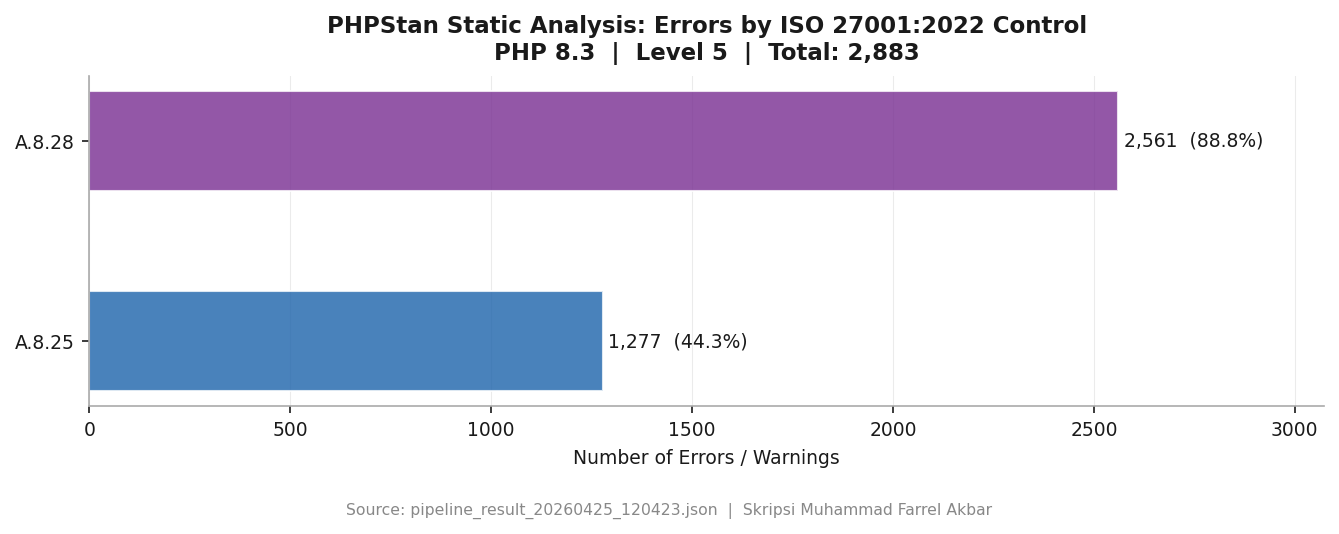
\includegraphics[width=1.0\textwidth]{contents/chapter-4/pipeline_chart_20260425_182849_4_phpstan_iso.png}
    \caption{Distribusi temuan PHPStan berdasarkan kontrol ISO/IEC 27001:2022 Annex A}
    \label{fig:phpstan-iso}
\end{figure}

Angka PHPStan yang tinggi justru menunjukkan manfaat nyata dari komponen validasi dalam \textit{pipeline} ini. Tanpa PHPStan, 2.871 potensi masalah tipe dan kompatibilitas ini tidak akan terdeteksi sampai kode dijalankan di lingkungan produksi, sesuai dengan temuan Strobl et al. \cite{strobl2020automated} tentang pentingnya jaminan kualitas otomatis dalam transformasi kode skala besar.

% ============================================================
\section{Status Kepatuhan ISO/IEC 27001:2022}
% ============================================================

Berdasarkan pemetaan yang dilakukan oleh \texttt{iso\_mapper.py}, status kepatuhan terhadap enam kontrol ISO/IEC 27001:2022 yang dipetakan adalah sebagaimana ditunjukkan pada Tabel \ref{tab:iso-status}.

\begin{table}[h]
\centering
\caption{Status kepatuhan ISO/IEC 27001:2022 hasil \textit{pipeline} pada dataset FT UGM}
\label{tab:iso-status}
\begin{tabularx}{\textwidth}{|l|l|X|l|}
\hline
\textbf{Kontrol} & \textbf{Judul} & \textbf{Dasar Penilaian} & \textbf{Status} \\
\hline
A.5.17 & \textit{Authentication Information} & Tidak ada temuan \textit{hardcoded credentials} & \texttt{COMPLIANT} \\
\hline
A.8.24 & \textit{Use of Cryptography} & Tidak ada temuan penggunaan \texttt{md5()}/\texttt{sha1()} untuk kata sandi & \texttt{COMPLIANT} \\
\hline
A.8.25 & \textit{Secure Development Lifecycle} & 1.266 temuan PHPStan (masalah kompatibilitas dan kualitas kode) & \texttt{NON\_COMPLIANT} \\
\hline
A.8.26 & \textit{Application Security Requirements} & 1 temuan SQL Injection dari Semgrep & \texttt{NON\_COMPLIANT} \\
\hline
A.8.28 & \textit{Secure Coding} & Temuan Semgrep aktif dan 2.549 ERROR PHPStan & \texttt{NON\_COMPLIANT} \\
\hline
A.8.29 & \textit{Security Testing in Development} & 10 temuan SSRF dari Semgrep & \texttt{PARTIAL} \\
\hline
\end{tabularx}
\end{table}

Status keseluruhan adalah \texttt{NON\_COMPLIANT}. Ini bukan hasil yang mengejutkan mengingat kondisi kode warisan yang dianalisis; justru ini adalah gambaran yang jujur tentang postur keamanan aplikasi sebelum dilakukan remediasi manual.

Dua kontrol yang berstatus \texttt{COMPLIANT}, yaitu A.5.17 dan A.8.24, perlu dipahami dalam konteks yang tepat. Status ini berarti \textit{ruleset} Semgrep yang digunakan tidak menghasilkan temuan yang dipetakan ke kedua kontrol tersebut, bukan berarti kode bebas dari masalah autentikasi atau kriptografi secara absolut.

Kontrol A.8.29 berstatus \texttt{PARTIAL} karena \textit{pipeline} sudah menjalankan pengujian keamanan otomatis sebagai bagian dari proses, yang memenuhi sebagian persyaratan kontrol ini. Namun masih ada temuan terbuka, sehingga kontrol belum sepenuhnya terpenuhi. Laporan kepatuhan ini dihasilkan secara otomatis dan dapat langsung digunakan sebagai dokumentasi audit ISO/IEC 27001:2022 \cite{iso27001_2022}.

% ============================================================
\section{Hasil Komparasi Lima Model LLM (Kondisi A)}
% ============================================================

Eksperimen Kondisi A dijalankan dengan \textit{prompt} yang identik untuk semua model (\textit{zero-shot}), 11 temuan Semgrep \textit{pre-scan} sebagai masukan, 3 \textit{run} per temuan per model, dan \textit{temperature} 0,1. Total percobaan adalah 165 (33 per model). Semua model dijalankan secara lokal melalui Ollama tanpa modifikasi.

\subsection{Format Compliance Rate}

Gambar \ref{fig:format-compliance-a} menunjukkan \textit{format compliance rate} untuk masing-masing model pada Kondisi A.

\begin{figure}[h]
    \centering
    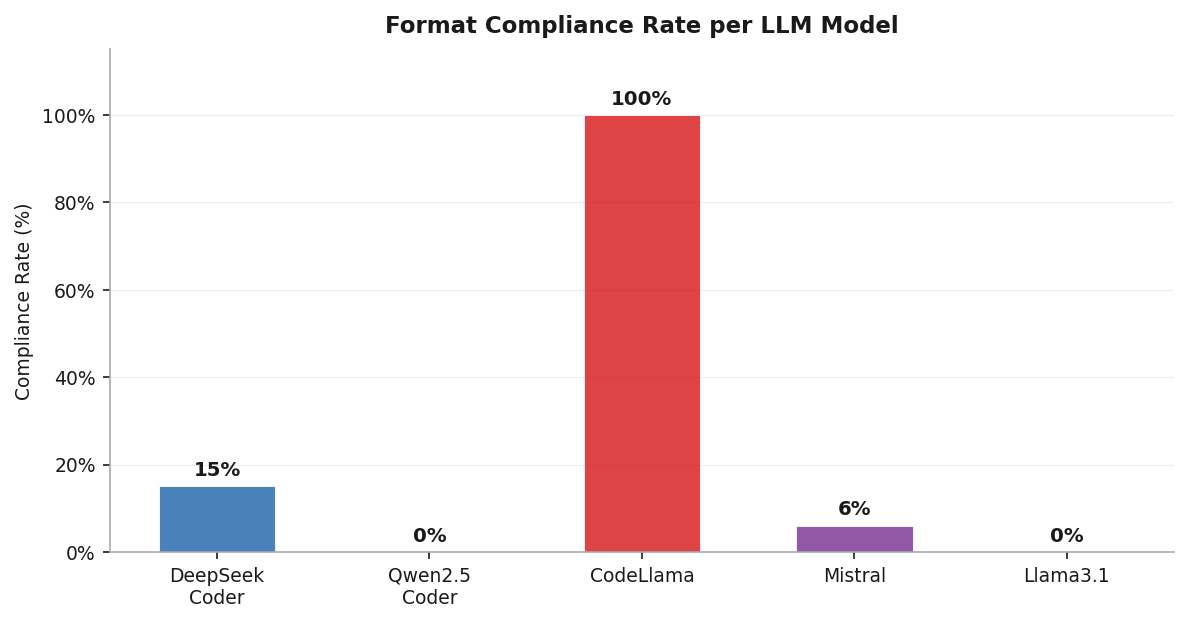
\includegraphics[width=1.0\textwidth]{contents/chapter-4/llm_chart_20260425_212836_2_format_compliance.png}
    \caption{\textit{Format compliance rate} kelima model LLM pada Kondisi A (\textit{zero-shot}, \textit{prompt} identik)}
    \label{fig:format-compliance-a}
\end{figure}

CodeLlama adalah satu-satunya model yang secara konsisten mengikuti format instruksi \textit{prompt} di semua 33 percobaan (100\%). DeepSeek Coder mengikuti format di 5 dari 33 percobaan (15\%). Mistral mengikuti format di 2 dari 33 percobaan (6\%). Qwen2.5-Coder dan Llama 3.1 tidak menghasilkan satu pun respons yang memenuhi ketiga elemen format sekaligus.

\subsection{Syntax Validity Rate}

Gambar \ref{fig:syntax-validity-a} menunjukkan \textit{syntax validity rate} dan \textit{code block extraction rate} untuk masing-masing model.

\begin{figure}[h]
    \centering
    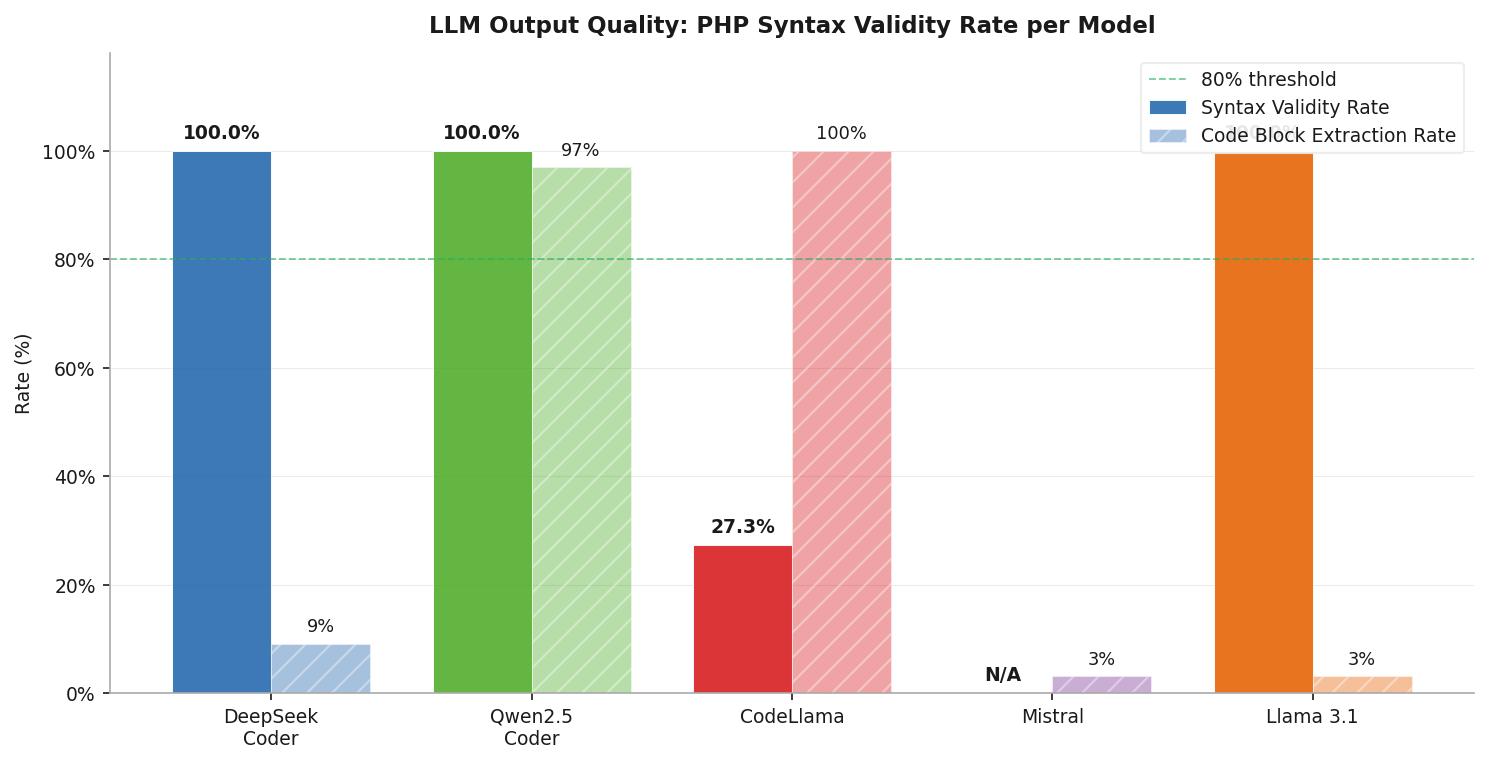
\includegraphics[width=1.0\textwidth]{contents/chapter-4/llm_quality_chart_20260425_205434.png}
    \caption{\textit{Syntax validity rate} dan \textit{code block extraction rate} kelima model LLM pada Kondisi A}
    \label{fig:syntax-validity-a}
\end{figure}

Hasilnya memperlihatkan gambaran yang berlawanan dengan metrik format. CodeLlama yang memiliki \textit{format compliance} 100\% ternyata hanya menghasilkan kode PHP yang \textit{valid} secara sintaksis pada 
9 dari 33 blok kode yang berhasil diekstraksi 
($SVR = 27{,}3\%$). Ini berarti 24 dari 33 blok kode CodeLlama mengandung \textit{parse error}.

Sebaliknya, Qwen2.5-Coder yang memiliki \textit{format compliance} 0\% berhasil mengekstraksi blok kode PHP dari 32 dari 33 percobaan (97\%), dan seluruh 32 blok kode tersebut lolos pemeriksaan \texttt{php -l} 
($SVR = 100\%$). Model ini mengabaikan instruksi format sepenuhnya, tetapi secara konsisten menghasilkan kode yang berkualitas baik.

Mistral berhasil mengekstraksi 1 blok kode dari 33 percobaan, tetapi blok tersebut tidak lolos \texttt{php -l} (0\% validitas). DeepSeek Coder dan Llama 3.1 masing-masing mengekstraksi 3 dan 1 blok dengan validitas 100\%, namun jumlah sampel yang terlalu kecil membuat angka ini tidak representatif secara statistik.

\subsection{Statistik Ringkasan}

Gambar \ref{fig:stats-table-a} merangkum statistik lengkap untuk kelima model pada Kondisi A.

\begin{figure}[h]
    \centering
    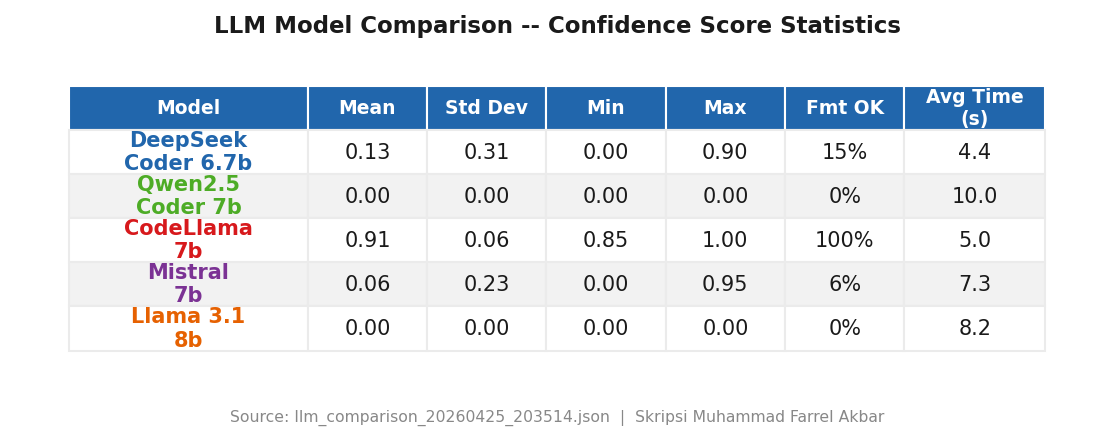
\includegraphics[width=\textwidth]{contents/chapter-4/llm_chart_20260425_212836_4_stats_table.png}
    \caption{Statistik lengkap komparasi kelima model LLM pada Kondisi A}
    \label{fig:stats-table-a}
\end{figure}

CodeLlama memiliki \textit{confidence score} rata-rata $\bar{C}_m = 0{,}909$ (0,909) dengan standar deviasi yang relatif kecil $\sigma_m = 0{,}054$ (0,054), mencerminkan konsistensi yang tinggi. Namun konsistensi ini tidak berkorelasi dengan kualitas kode: 72,7\% kode CodeLlama tidak \textit{valid} secara sintaksis. Ini mengkonfirmasi bahwa \textit{confidence score self-reported} bukan ukuran kualitas kode.

Qwen2.5-Coder memiliki \textit{confidence score} rata-rata $\bar{C}_m = 0{,}000$ (0,000) karena tidak pernah menghasilkan baris \texttt{CONFIDENCE: N}. Ketidakhadiran skor ini bukan tanda ketidakmampuan, melainkan refleksi dari gaya respons model yang mengabaikan instruksi format sambil tetap mengerjakan tugas utama dengan sangat baik. Waktu inferensi Qwen2.5-Coder (10,0 detik) paling lama dibanding model lain, kemungkinan karena model ini menghasilkan respons yang lebih panjang dan detail.

\subsection{Analisis Kualitatif: Perbandingan Respons terhadap Temuan SQL Injection}

Untuk memperlihatkan perbedaan perilaku model secara konkret, berikut perbandingan respons CodeLlama dan Qwen2.5-Coder terhadap temuan SQL Injection yang sama dari \texttt{Output.php} baris 768. Kode yang dikirimkan ke model adalah sebagai berikut:

\begin{small}
\begin{verbatim}
$uri .= '?'.$_SERVER['QUERY_STRING'];
$cache_path .= md5(
    $CI->config->item('base_url')
    .$CI->config->item('index_page')
    .ltrim($uri, '/'));

if ( ! @unlink($cache_path)) {
    log_message('error',
        'Unable to delete cache file for '.$uri);
    return FALSE;
}
\end{verbatim}
\end{small}

\textbf{Respons CodeLlama:}

\begin{small}
\begin{verbatim}
VULNERABILITY: SQL Injection Vulnerability

The vulnerability is caused by the manual construction
of an SQL string, which allows user-controlled data
to be incorporated into the query. ...

SECURE PHP 8.x REPLACEMENT:
```php
$uri = $_SERVER['QUERY_STRING'];
$cache_path = md5(
    $CI->config->item('base_url')
    .$CI->config->item('index_page')
    .ltrim($uri, '/'));
if ( ! @unlink($cache_path)) {
    log_message('error',
        'Unable to delete cache file for '.$uri);
    return FALSE;
}
(blok kode tidak ditutup, php -l gagal)
\end{verbatim}
\end{small}

\textbf{Respons Qwen2.5-Coder:}

\begin{small}
\begin{verbatim}
### Explanation of Vulnerability
...
Here's the corrected PHP 8.x code:
```php
$uri .= '?' . urlencode($_SERVER['QUERY_STRING']);
$cache_path .= md5(
    $CI->config->item('base_url')
    . $CI->config->item('index_page')
    . ltrim($uri, '/'));

if (!@unlink($cache_path)) {
    log_message('error',
        'Unable to delete cache file for '
        . urlencode($uri));
    return FALSE;
}
```
\end{verbatim}
\end{small}

Dari perbandingan ini terlihat beberapa perbedaan yang signifikan. CodeLlama mengidentifikasi kerentanan dengan benar tapi solusinya tidak tepat: model hanya mengubah cara penulisan kode tanpa benar-benar mengatasi masalahnya. Kode yang dihasilkan masih menggunakan \texttt{\$\_SERVER['QUERY\_STRING']} secara langsung tanpa sanitasi apapun.

Qwen2.5-Coder menunjukkan pemahaman kontekstual yang lebih dalam. Model ini menyadari bahwa meskipun Semgrep menandainya sebagai SQL Injection, kode tersebut sebenarnya membangun \textit{cache path}, bukan kueri SQL. Saran perbaikannya menggunakan \texttt{urlencode()} untuk menghindari karakter berbahaya dalam \textit{path}. Secara semantik ini lebih tepat, meski solusi yang ideal tetap perlu ditinjau oleh pengembang yang memahami konteks penuh aplikasi.

\subsection{Trade-off dan Implikasinya}

Dari keseluruhan hasil Kondisi A, terdapat \textit{trade-off} yang jelas antara kepatuhan format dan kualitas kode. Model yang paling patuh pada instruksi format (CodeLlama, 100\%) menghasilkan kode dengan tingkat sintaksis \textit{error} tertinggi (72,7\% kode tidak valid). Model yang menghasilkan kode paling berkualitas (Qwen2.5-Coder, 97\% \textit{extraction rate} dan 100\% validitas) mengabaikan instruksi format sepenuhnya.

Temuan ini memiliki implikasi langsung untuk desain sistem berbasis LLM lokal: metrik kualitas kode (\textit{syntax validity rate}) adalah indikator yang jauh lebih relevan dibandingkan metrik kepatuhan format. Sistem evaluasi yang hanya mengandalkan kepatuhan format akan salah menilai model mana yang lebih berguna secara praktis.

\textit{Trade-off} ini juga menunjukkan bahwa kondisi \textit{zero-shot} dengan \textit{prompt} identik mungkin tidak optimal untuk semua model secara bersamaan. Ini menjadi motivasi utama untuk Kondisi B, di mana setiap model menerima \textit{prompt} yang dioptimasi berdasarkan karakteristik dan kelemahan yang terobservasi pada Kondisi A.

% ============================================================
\section{Hasil Komparasi Lima Model LLM (Kondisi B)}
% ============================================================

Kondisi B dirancang untuk mengatasi kelemahan spesifik setiap model yang teridentifikasi pada Kondisi A. Setiap model menerima \textit{prompt} yang berbeda melalui metode \texttt{\_build\_optimized\_chat\_messages()} di \texttt{ai\_engine.py}, sementara parameter eksperimen lainnya tetap sama: 11 temuan Semgrep yang sama, 3 \textit{run} per temuan per model, dan \textit{temperature} 0,1.

Strategi optimasi per model dirumuskan berdasarkan pola kegagalan Kondisi A. Qwen2.5-Coder menerima \textit{prompt} yang lebih longgar tanpa tuntutan format ketat karena kualitas kodenya sudah baik. DeepSeek Coder menerima instruksi yang lebih pendek dan langsung untuk mengurangi kompleksitas yang diduga menjadi penyebab rendahnya \textit{extraction rate}. Mistral menerima satu contoh \textit{few-shot} konkret untuk menunjukkan format keluaran yang diharapkan. Llama 3.1 menerima instruksi berbasis \textit{role-playing} eksplisit dengan langkah-langkah bernomor. CodeLlama mempertahankan format Kondisi A dengan tambahan instruksi eksplisit agar menghasilkan kode PHP yang \textit{valid} secara sintaksis.

\subsection{Format Compliance Rate}

Gambar \ref{fig:format-compliance-b} menunjukkan \textit{format compliance rate} untuk masing-masing model pada Kondisi B.

\begin{figure}[h]
    \centering
    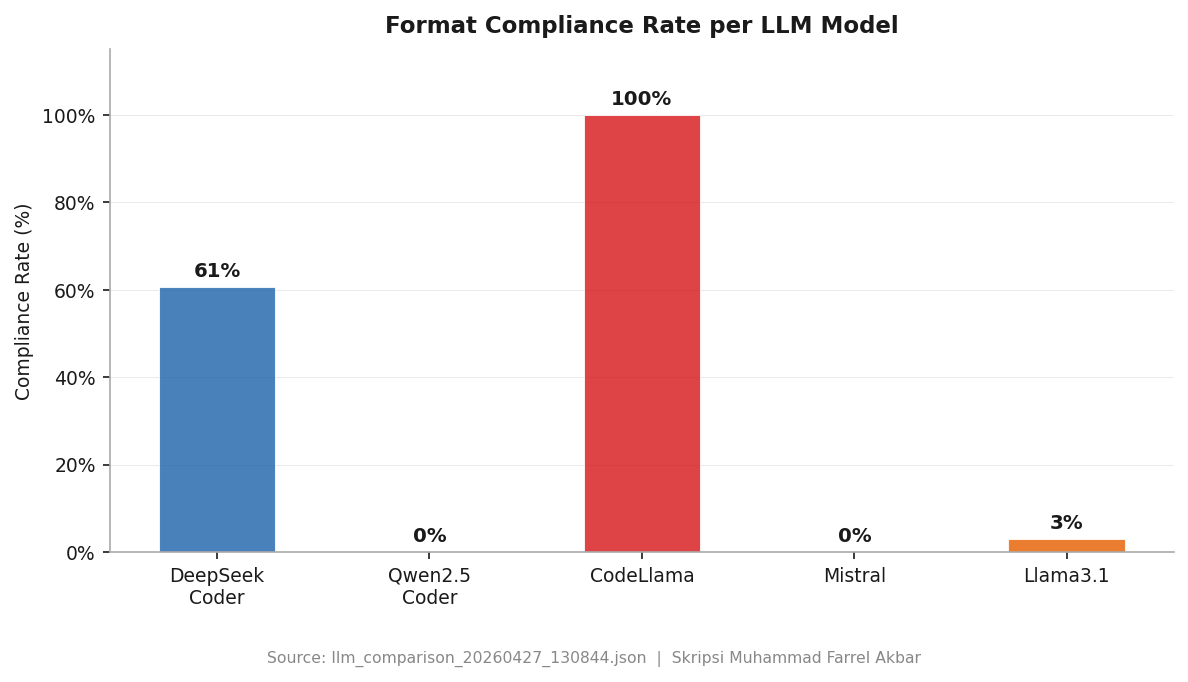
\includegraphics[width=0.85\textwidth]{contents/chapter-4/llm_chart_20260427_140238_2_format_compliance.png}
    \caption{\textit{Format compliance rate} kelima model LLM pada Kondisi B (\textit{prompt} dioptimasi per model)}
    \label{fig:format-compliance-b}
\end{figure}

DeepSeek Coder mencatat peningkatan yang paling signifikan, dari 15\% pada Kondisi A menjadi 61\% pada Kondisi B. Ini mengkonfirmasi bahwa model ini sangat sensitif terhadap kompleksitas instruksi: \textit{prompt} yang lebih pendek dan langsung secara substansial meningkatkan kemampuannya mengikuti format. CodeLlama mempertahankan \textit{format compliance} 100\% seperti pada Kondisi A. Sebaliknya, Mistral mengalami regresi dari 6\% menjadi 0\%, dan Llama 3.1 hanya naik tipis dari 0\% menjadi 3\% (1 dari 33 \textit{run}).
\newpage
\subsection{Syntax Validity Rate}

Gambar \ref{fig:syntax-validity-b} menunjukkan \textit{syntax validity rate} dan \textit{code block extraction rate} pada Kondisi B.

\begin{figure}[h]
    \centering
    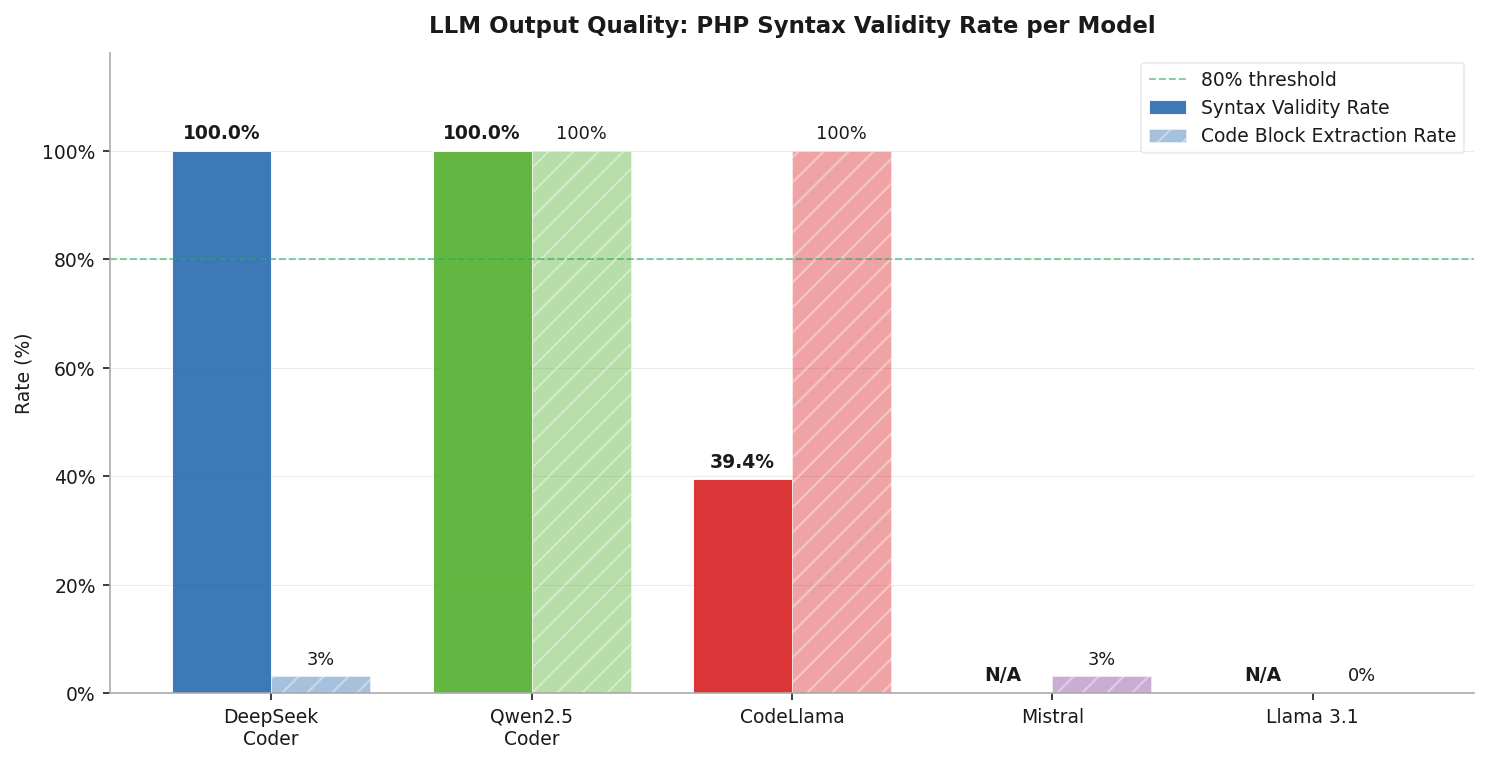
\includegraphics[width=1.0\textwidth]{contents/chapter-4/llm_quality_chart_20260427_133011.png}
    \caption{\textit{Syntax validity rate} dan \textit{code block extraction rate} kelima model LLM pada Kondisi B}
    \label{fig:syntax-validity-b}
\end{figure}

Qwen2.5-Coder mempertahankan posisinya sebagai model dengan kualitas kode terbaik: \textit{extraction rate} naik dari 97\% menjadi 100\% dan \textit{syntax validity} tetap 100\%. CodeLlama menunjukkan perbaikan parsial pada \textit{syntax validity}, dari 27,3\% menjadi 39,4\%, meskipun masih jauh dari ambang batas yang dapat diandalkan. DeepSeek Coder mengalami penurunan \textit{extraction rate} dari 9\% menjadi 3\% meskipun \textit{format compliance}-nya meningkat, yang menunjukkan adanya \textit{trade-off} antara kepatuhan format dan kemampuan menghasilkan blok kode. Mistral dan Llama 3.1 secara efektif tidak menghasilkan kode yang dapat digunakan pada Kondisi B.
\newpage
\subsection{Statistik Ringkasan}

Gambar \ref{fig:stats-table-b} merangkum statistik lengkap untuk 
kelima model pada Kondisi B.

\begin{figure}[h]
    \centering
    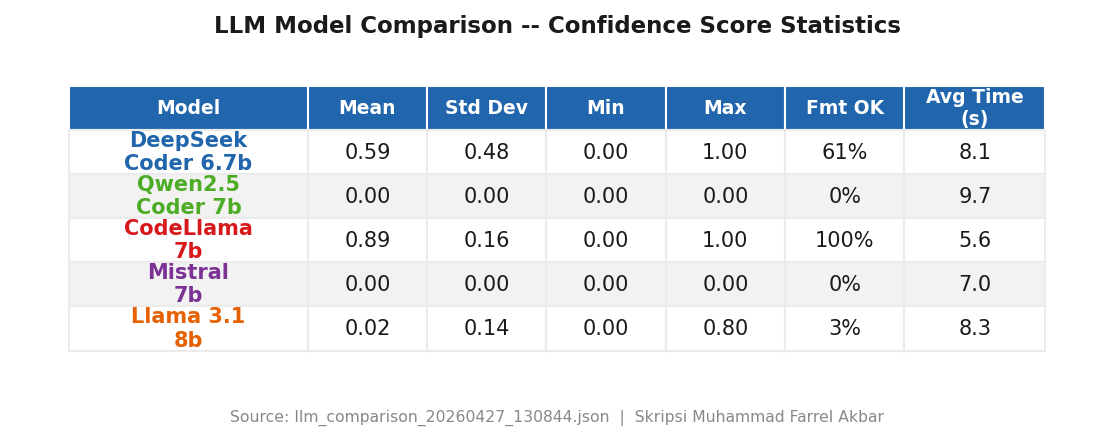
\includegraphics[width=\textwidth]{contents/chapter-4/llm_chart_20260427_140238_4_stats_table.png}
    \caption{Statistik lengkap komparasi kelima model LLM pada Kondisi B}
    \label{fig:stats-table-b}
\end{figure}

DeepSeek Coder mencatat peningkatan \textit{mean confidence} yang 
paling mencolok, dari $\bar{C}_m = 0{,}132$ pada Kondisi A menjadi 
$\bar{C}_m = 0{,}588$ pada Kondisi B. 
Variansi yang tinggi ($\sigma_m = 0{,}477$) menunjukkan bahwa 
skor ini tidak stabil: sebagian \textit{run} menghasilkan skor 
mendekati 1,0 sementara sebagian lainnya tetap di 0,0. Pola ini 
konsisten dengan \textit{format compliance} 61\%: hanya sekitar 
dua pertiga percobaan yang benar-benar menulis baris 
\texttt{CONFIDENCE:}, sedangkan sisanya tidak sama sekali.

CodeLlama mempertahankan \textit{mean confidence} yang tinggi 
($\bar{C}_m = 0{,}894$) dengan standar deviasi yang kecil 
($\sigma_m = 0{,}162$), mencerminkan konsistensi yang sama seperti 
pada Kondisi A. Angka ini mungkin 
tampak meyakinkan, tetapi perlu diingat bahwa \textit{syntax 
validity rate} CodeLlama hanya 39,4\%: artinya model ini sangat 
yakin dengan jawabannya meski lebih dari separuh kode yang 
dihasilkannya tidak lolos \texttt{php -l}. Ini kembali 
mengkonfirmasi bahwa \textit{confidence score self-reported} tidak 
bisa dijadikan proksi kualitas kode.

Qwen2.5-Coder, Mistral, dan Llama 3.1 mencatat \textit{mean 
confidence} 0,000 karena tidak satu pun respons mereka yang 
menulis baris \texttt{CONFIDENCE:} dalam format yang dapat 
di-\textit{parse}. Khusus untuk Qwen2.5-Coder, ketiadaan skor ini 
justru tidak mencerminkan kualitas yang buruk: model ini tetap 
menghasilkan kode dengan \textit{syntax validity} 100\% di Kondisi 
B, sama seperti Kondisi A. Ketiadaan skor kepercayaan semata-mata 
mencerminkan gaya respons model yang mengabaikan instruksi format 
sambil tetap mengerjakan tugas utamanya dengan baik.

Secara keseluruhan, pola yang sama dengan Kondisi A terulang: 
tidak ada korelasi yang dapat diandalkan antara tingginya 
\textit{confidence score} dan kualitas kode yang dihasilkan. 
Ini memperkuat argumen bahwa untuk sistem berbasis LLM lokal 
berukuran kecil hingga menengah, \textit{syntax validity rate} 
tetap menjadi metrik evaluasi yang lebih sahih dibandingkan 
\textit{confidence score self-reported}.
% ============================================================
\section{Perbandingan Kondisi A dan Kondisi B}
% ============================================================

Tabel \ref{tab:ab-comparison} merangkum perbandingan metrik utama antara Kondisi A dan Kondisi B untuk kelima model.

\begin{table}[h]
\centering
\caption{Perbandingan metrik utama Kondisi A vs Kondisi B untuk kelima model LLM}
\label{tab:ab-comparison}
\resizebox{\textwidth}{!}{%
\begin{tabular}{|l|c|c|c|c|c|c|}
\hline
\multirow{2}{*}{\textbf{Model}} &
  \multicolumn{2}{c|}{\textbf{Format Compliance}} &
  \multicolumn{2}{c|}{\textbf{Extraction Rate}} &
  \multicolumn{2}{c|}{\textbf{Syntax Validity}} \\
\cline{2-7}
 & \textbf{Kond.~A} & \textbf{Kond.~B} &
   \textbf{Kond.~A} & \textbf{Kond.~B} &
   \textbf{Kond.~A} & \textbf{Kond.~B} \\
\hline
DeepSeek Coder 6.7b
  & 15\%  & \textbf{61\%} $\uparrow$
  & 9\%   & 3\% $\downarrow$
  & 100\% & 100\% \\
\hline
Qwen2.5-Coder 7b
  & 0\%   & 0\%
  & 97\%  & \textbf{100\%} $\uparrow$
  & 100\% & 100\% \\
\hline
CodeLlama 7b
  & 100\% & 100\%
  & 100\% & 100\%
  & 27\%  & \textbf{39\%} $\uparrow$ \\
\hline
Mistral 7b
  & 6\%   & 0\% $\downarrow$
  & 3\%   & 3\%
  & 0\%   & 0\% \\
\hline
Llama 3.1 8b
  & 0\%   & 3\% $\uparrow$
  & 3\%   & 0\% $\downarrow$
  & 100\% & 0\% $\downarrow$ \\
\hline
\end{tabular}%
}
\end{table}

Dari perbandingan ini, ada tiga pola utama yang dapat diidentifikasi.

\textbf{Pertama}, optimasi \textit{prompt} hanya bekerja signifikan pada model yang memiliki kapabilitas \textit{instruction-following} dasar yang memadai. DeepSeek Coder adalah satu-satunya model yang menunjukkan peningkatan substansial pada \textit{format compliance} (dari 15\% menjadi 61\%), mengkonfirmasi bahwa model ini peka terhadap kompleksitas instruksi: bukan tidak mampu mengikuti format, tapi terbebani oleh instruksi yang terlalu berlapis pada Kondisi A.

\textbf{Kedua}, strategi \textit{few-shot} untuk Mistral memberikan hasil yang berlawanan dari yang diharapkan: \textit{format compliance} justru turun dari 6\% menjadi 0\%. Fenomena ini, di mana contoh \textit{few-shot} justru mengalihkan model dari mengerjakan tugas aslinya, konsisten dengan temuan dalam literatur yang menunjukkan bahwa teknik \textit{prompt engineering} yang efektif untuk model besar tidak selalu dapat diterapkan langsung pada model berukuran kecil hingga menengah \cite{akuthota2023vulnerability}.

\textbf{Ketiga}, keterbatasan CodeLlama dalam menghasilkan kode PHP yang \textit{valid} secara sintaksis bersifat struktural, bukan instruksional. Meskipun instruksi eksplisit untuk memverifikasi sintaks sebelum menulis kode memberikan perbaikan parsial (dari 27\% menjadi 39\%), sebagian besar kode yang dihasilkan masih mengandung \textit{parse error}. Ini menunjukkan bahwa masalah ini berakar pada representasi internal model terhadap sintaks PHP 8.x, bukan pada cara instruksi diformulasikan.

Secara keseluruhan, hasil Kondisi B mempertegas kesimpulan dari Kondisi A bahwa pilihan model adalah faktor yang lebih menentukan dibandingkan strategi \textit{prompt} dalam konteks analisis keamanan kode PHP menggunakan LLM lokal berukuran kecil hingga menengah. Qwen2.5-Coder secara konsisten menghasilkan kode yang paling berkualitas di kedua kondisi, terlepas dari format \textit{prompt} yang diberikan.

% ============================================================
\section{Optimasi Parameter Qwen2.5-Coder (Kondisi C)}
% ============================================================

Setelah Kondisi A dan B mengidentifikasi Qwen2.5-Coder sebagai 
model dengan kualitas kode terbaik, Kondisi C mengevaluasi apakah 
performa model ini dapat ditingkatkan lebih lanjut melalui variasi 
dua parameter inferensi: \textit{temperature} dan 
\textit{context window}. Eksperimen ini menggunakan input, jumlah 
\textit{run}, dan \textit{prompt} yang identik dengan Kondisi A, 
hanya parameter yang diuji yang berbeda.

Gambar \ref{fig:kondisi-c} menunjukkan perbandingan ketiga metrik 
utama di semua variasi parameter.

\begin{figure}[h]
    \centering
    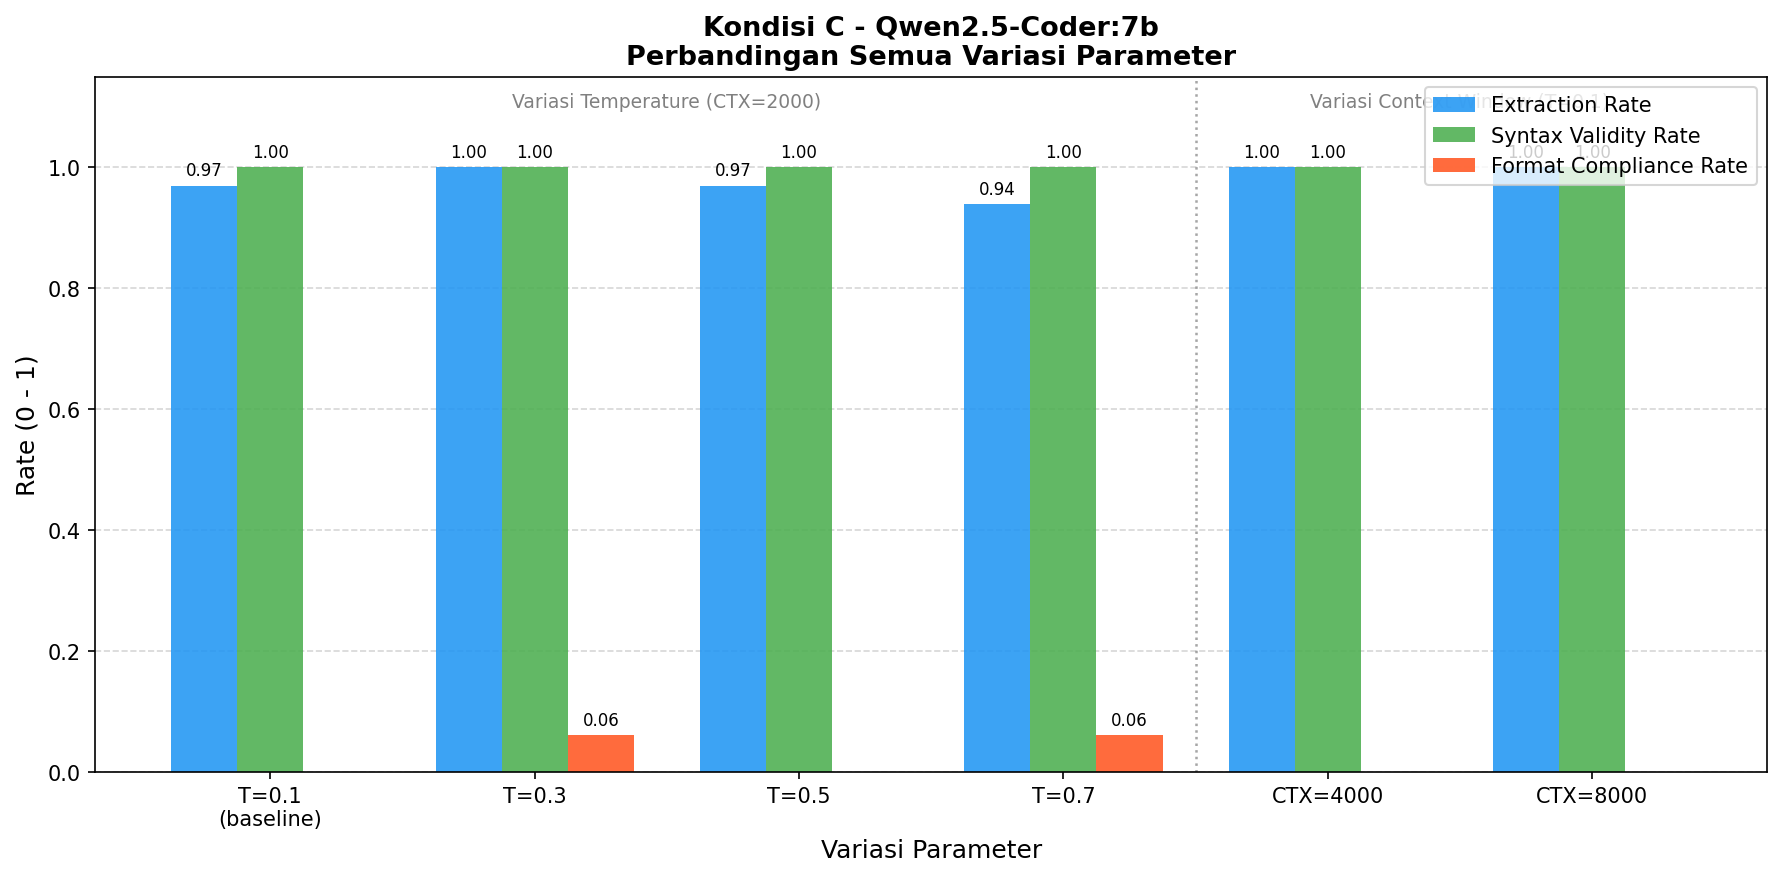
\includegraphics[width=\textwidth]{contents/chapter-4/llm_chart_kondisi_c_parameter_comparison.png}
    \caption{Perbandingan metrik Qwen2.5-Coder pada variasi 
    \textit{temperature} dan \textit{context window} (Kondisi C)}
    \label{fig:kondisi-c}
\end{figure}

\subsection{Pengaruh Temperature}

Pada variasi \textit{temperature}, \textit{syntax validity rate} 
bertahan di 100\% di semua nilai yang diuji (0,1 hingga 0,7). 
Ini menunjukkan bahwa kemampuan Qwen2.5-Coder menghasilkan kode 
PHP yang \textit{valid} secara sintaksis tidak terdegradasi meski 
\textit{temperature} dinaikkan secara signifikan.

\textit{Extraction rate} justru sedikit menurun seiring naiknya 
\textit{temperature}: dari 100\% di T=0,3 menjadi 94\% di T=0,7. 
Ini konsisten dengan ekspektasi teoritis bahwa \textit{temperature} 
tinggi meningkatkan variabilitas respons, sehingga sebagian kecil 
respons tidak lagi mengandung blok kode yang dapat diekstraksi.

\textit{Format compliance} memperlihatkan pola yang tidak monoton: 
muncul di T=0,3 (6\%) dan T=0,7 (6\%), tetapi kembali ke 0\% di 
T=0,5. Kemunculan \textit{format compliance} yang tidak konsisten 
ini mengindikasikan bahwa kepatuhan format pada Qwen2.5-Coder 
lebih dipengaruhi oleh variabilitas stokastik daripada perubahan 
\textit{temperature} secara sistematis.

\subsection{Pengaruh Context Window}

Pada variasi \textit{context window}, baik CTX=4000 maupun 
CTX=8000 menghasilkan \textit{extraction rate} dan 
\textit{syntax validity rate} 100\%, sedikit di atas baseline 
CTX=2000 yang memiliki \textit{extraction rate} 97\%. 
\textit{Format compliance} tetap 0\% di kedua variasi.

Peningkatan \textit{extraction rate} dari 97\% ke 100\% pada 
konteks yang lebih besar mengindikasikan bahwa dengan informasi 
kode yang lebih lengkap, model lebih konsisten menghasilkan blok 
kode dalam setiap respons. Namun peningkatan ini marginal dan 
tidak mengubah karakteristik utama model.

\subsection{Implikasi Kondisi C}

Kondisi C menunjukkan bahwa karakteristik Qwen2.5-Coder lebih 
ditentukan oleh arsitektur modelnya daripada konfigurasi parameter. 
Kualitas kode yang dihasilkan sangat stabil di semua variasi 
parameter yang diuji. Dalam penerapan nyata, hal ini berarti operator tidak perlu melakukan 
penyesuaian parameter yang ekstensif untuk mendapatkan keluaran 
berkualitas dari model ini. Konfigurasi \textit{default} (T=0,1, CTX=2000) sudah 
memberikan hasil yang hampir optimal, sementara peningkatan 
\textit{context window} ke 4000 atau 8000 karakter dapat 
memberikan sedikit keuntungan tambahan pada kode yang lebih panjang.

% ============================================================
\section{Analisis Dependensi Composer (FT UGM)}
% ============================================================

Modul \texttt{composer\_analyzer.py} membaca berkas \texttt{composer.json} 
pada direktori \textit{root} repositori FT UGM dan memeriksa kompatibilitas 
setiap dependensi terhadap PHP 8.x menggunakan data dari Packagist. 
Terdapat 5 dependensi yang teridentifikasi, dengan hasil sebagaimana 
ditunjukkan pada Tabel \ref{tab:composer-ft}.

\begin{table}[h]
\centering
\caption{Status kompatibilitas PHP 8.x dependensi \textit{composer} FT UGM}
\label{tab:composer-ft}
\begin{tabularx}{\textwidth}{|l|l|X|}
\hline
\textbf{Package} & \textbf{Versi} & \textbf{Status} \\
\hline
\texttt{vlucas/phpdotenv} & \texttt{\^{}5.4} & \texttt{SAFE} \\
\hline
\texttt{phpoffice/phpspreadsheet} & \texttt{\^{}1.12} & \texttt{SAFE} \\
\hline
\texttt{firebase/php-jwt} & \texttt{\^{}6.10} & \texttt{SAFE} \\
\hline
\texttt{ngekoding/google-login} & \texttt{\^{}1.0} & \texttt{MANUAL REVIEW} \\
\hline
\texttt{chriskacerguis/codeigniter-restserver} & \texttt{\^{}3.1} & \texttt{MANUAL REVIEW} \\
\hline
\end{tabularx}
\end{table}

Tiga dari lima dependensi (\texttt{phpdotenv}, \texttt{phpspreadsheet}, 
\texttt{firebase/\allowbreak php-jwt}) berstatus \texttt{SAFE}, artinya versi yang 
dikonfigurasi di \texttt{composer.json} sudah deklaratif mendukung PHP 8.x. 
Dua dependensi lainnya berstatus \texttt{MANUAL REVIEW}: 
\texttt{ngekoding/\allowbreak google-login} merupakan paket dengan aktivitas pemeliharaan 
rendah sehingga kompatibilitas PHP 8.x-nya tidak dapat diverifikasi secara 
otomatis, sementara \texttt{chriskacerguis/\allowbreak codeigniter-restserver} merupakan 
ekstensi pihak ketiga untuk CodeIgniter 3.x yang diketahui tidak memiliki 
dukungan resmi untuk PHP 8.x dan perlu diganti atau diperbarui secara manual 
sebelum deployment ke lingkungan PHP 8.3.

% ============================================================
\section{Diskusi dan Keterbatasan}
% ============================================================

\subsection{Keterbatasan Dataset}

Dataset yang digunakan terdiri dari satu aplikasi berbasis CodeIgniter 3.x milik FT UGM. Dari 245 \textit{file}, 237 diklasifikasikan sebagai \textit{unknown} oleh Rector karena merupakan \textit{file framework} CodeIgniter yang tidak mengandung pola yang perlu ditransformasi. Hal ini membatasi seberapa jauh hasil penelitian ini bisa digeneralisasi ke jenis aplikasi PHP lain, terutama yang tidak menggunakan \textit{framework} atau yang menggunakan \textit{framework} berbeda.

Dari sisi \textit{input} eksperimen LLM, 10 dari 11 temuan adalah SSRF yang berasal dari satu pola kode yang berulang di \texttt{Output.php}. Homogenitas \textit{input} ini berarti eksperimen komparasi pada dasarnya menguji respons model terhadap dua jenis kerentanan dengan variasi terbatas. Hasil komparasi perlu diinterpretasikan dalam konteks keterbatasan ini.

\subsection{Keterbatasan Kompatibilitas PHP 8.4 dan PHP 8.5}

Eksperimen tambahan dilakukan untuk menguji \textit{pipeline} dengan 
target PHP 8.5 terhadap dataset CBT DTI UGM. Hasil menunjukkan dua 
masalah fundamental yang membatasi penerapan otomatis pada versi ini.

Pertama, Rector memperkenalkan \textit{syntax error} pada beberapa 
berkas inti CodeIgniter 3.x di direktori \texttt{system/}, khususnya 
\texttt{CodeIgniter.php}, \texttt{Output.php}, dan 
\texttt{Security.php}, karena \textit{ruleset} PHP 8.5 menerapkan 
transformasi yang tidak kompatibel dengan pola kode \textit{framework} 
lama. Kedua, akibat berkas \texttt{system/} yang rusak pasca-konversi, 
PHPStan tidak dapat me-\textit{resolve} kelas induk CodeIgniter seperti 
\texttt{CI\_Controller} dan \texttt{CI\_Model}, sehingga menghasilkan 
ribuan \textit{error} bertipe \textit{unknown class} yang merupakan 
\textit{false positive} kaskade. Total 6.137 \textit{error} PHPStan 
yang dihasilkan tidak representatif terhadap kualitas kode aplikasi 
yang sebenarnya.

Penyebab utama kegagalan ini bukan semata inkompatibilitas CI3 dengan 
PHP 8.5, melainkan \textit{ruleset} \texttt{UP\_TO\_PHP\_85} pada 
Rector yang masih bersifat eksperimental dan menerapkan transformasi 
yang terlalu agresif terhadap kode \textit{framework} lama. PHP 8.4 
diprediksi lebih \textit{feasible} dibanding PHP 8.5 karena 
\textit{ruleset}-nya sudah lebih matang dan perubahannya lebih 
konservatif, namun tetap memerlukan perbaikan manual pada pola 
\textit{dynamic property} CodeIgniter 3.x yang sudah sepenuhnya 
dihapus di PHP 8.4. PHP 8.3 tetap merupakan target migrasi otomatis 
yang paling realistis untuk basis kode CodeIgniter 3.x yang masih 
aktif digunakan.

Jalur yang realistis menuju PHP 8.5 adalah pembaruan \textit{framework} 
ke CodeIgniter 4 atau \textit{framework} modern lainnya yang sudah 
mendukung PHP 8.x secara \textit{native} — sebuah proses yang melampaui 
cakupan migrasi versi otomatis dan pada dasarnya merupakan penulisan 
ulang aplikasi. Oleh karena itu, PHP 8.3 ditetapkan sebagai versi 
target dalam penelitian ini sebagai pilihan yang dapat dicapai secara 
otomatis untuk aplikasi berbasis CodeIgniter 3.x.

\subsection{Keterbatasan Teknis Pipeline}

AI Engine hanya memproses temuan dengan prioritas 1--3 dan membatasi potongan kode yang dikirim ke model pada 2.000 karakter pertama. Untuk \textit{file} PHP yang panjang, konteks yang diterima model terpotong sehingga saran perbaikan mungkin tidak mempertimbangkan keseluruhan logika fungsi. Sebagaimana terlihat pada contoh respons Qwen2.5-Coder, model dapat membuat inferensi yang tepat tentang konteks kode meski dengan informasi yang terbatas, namun tidak selalu bisa dipastikan.

Selain itu, validasi menggunakan \texttt{php -l} hanya memeriksa kebenaran sintaksis, bukan kebenaran semantik. Kode yang lolos \texttt{php -l} bisa saja masih mengandung kerentanan yang tidak tertangani atau logika yang tidak ekuivalen dengan kode aslinya. Pengujian fungsional terhadap kode hasil perbaikan AI bukan bagian dari cakupan penelitian ini.

\subsection{Interpretasi Confidence Score}

Tidak ada korelasi yang jelas antara \textit{confidence score} yang dilaporkan model dan kualitas kode yang dihasilkan, baik pada Kondisi A maupun Kondisi B. CodeLlama melaporkan kepercayaan diri rata-rata lebih dari 90\% di kedua kondisi, tetapi mayoritas kode yang dihasilkannya tidak \textit{valid} secara sintaksis. Qwen2.5-Coder tidak melaporkan skor sama sekali tetapi menghasilkan kode yang hampir selalu berkualitas baik. Temuan ini konsisten dengan literatur yang menunjukkan bahwa model LLM berukuran kecil umumnya tidak terkalibrasi dengan baik dalam menilai \textit{output} mereka sendiri \cite{akuthota2023vulnerability}\cite{li2025iris}.
Dari ketiga metrik yang diukur $FCR$, \textit{extraction rate}, 
dan $SVR$, hanya $SVR$ yang secara konsisten mencerminkan 
kegunaan praktis model dalam konteks ini.

% ============================================================
\section{Studi Kasus 2: Sistem CBT DTI UGM}
% ============================================================

Studi kasus kedua menggunakan kode sumber aplikasi \textit{Computer-Based Test} 
(CBT) milik Direktorat Teknologi Informasi (DTI) Universitas Gadjah Mada. 
Aplikasi ini dibangun di atas \textit{framework} CodeIgniter 3 dengan persyaratan 
versi PHP $\geq$ 7.0, dan dikonversi ke target PHP 8.3. \textit{Pipeline} 
dijalankan terhadap direktori \texttt{application/} dengan mengeksklusi 
subdirektori \texttt{libraries/}, \texttt{third\_party/}, dan \texttt{tcpdf/} 
yang merupakan komponen \textit{framework} dan \textit{library} pihak ketiga, 
sehingga menghasilkan 183 \textit{file} PHP kustom sebagai masukan.

% ------------------------------------------------------------
\subsection{Hasil Konversi Rector}
% ------------------------------------------------------------

Rector dijalankan terhadap 183 \textit{file} PHP dengan target versi PHP 8.3. 
Dari jumlah tersebut, 158 \textit{file} berhasil dikonversi, 25 \textit{file} 
dilewati (\textit{skipped}), dan tidak ada \textit{file} yang gagal diproses. 
Tingkat konversi keseluruhan ($CR = 86{,}3\%$), sebagaimana ditunjukkan pada 
Gambar \ref{fig:rector-conversion-dti}.

\begin{figure}[h]
    \centering
    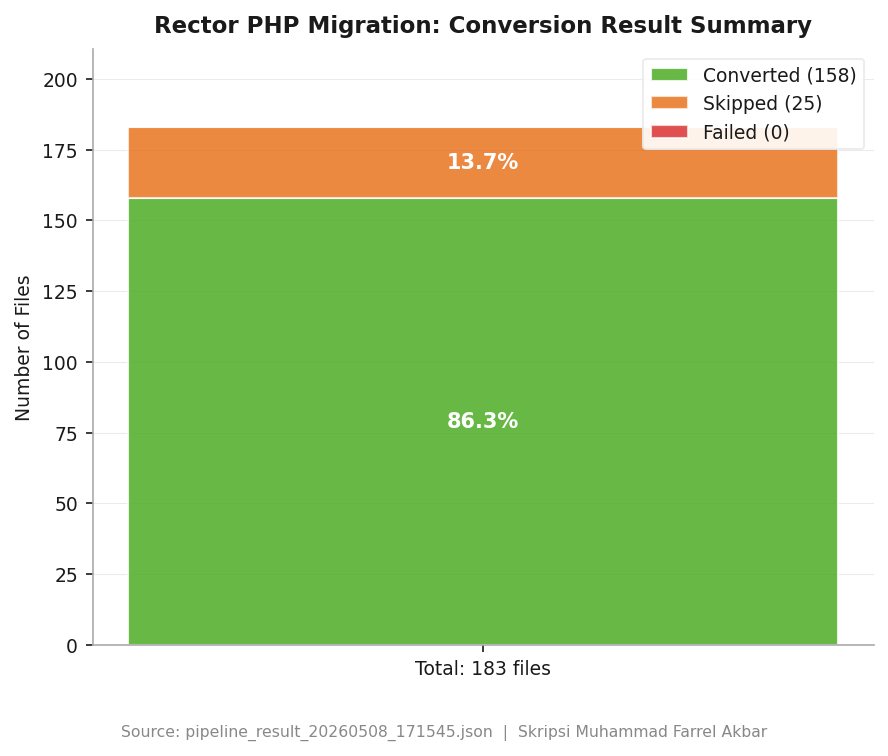
\includegraphics[width=0.8\textwidth]{contents/chapter-4/dti/pipeline_chart_20260509_074426_3_rector_conversion.png}
    \caption{Ringkasan hasil konversi Rector terhadap 183 \textit{file} PHP dataset CBT DTI UGM}
    \label{fig:rector-conversion-dti}
\end{figure}

Tingkat konversi yang lebih rendah dibanding studi kasus FT UGM (86,3\% vs 
97,6\%) disebabkan oleh proporsi \textit{file} yang dilewati yang lebih besar: 
25 dari 183 \textit{file} (13,7\%) tidak memerlukan transformasi apa pun karena 
kodenya sudah kompatibel dengan target PHP 8.3 atau tidak mengandung pola yang 
perlu ditangani oleh \textit{ruleset} Rector. Tidak adanya \textit{file} yang 
gagal diproses menunjukkan bahwa kode CBT DTI tidak mengandung konstruksi yang 
memicu \textit{bug} \texttt{FiberNodeScopeResolver} seperti yang ditemukan pada 
dataset FT UGM.

Seluruh \textit{file} pada direktori \texttt{output/} diuji validitas 
sintaksisnya menggunakan perintah \texttt{php -l} dan tidak ditemukan 
\textit{parse error}, sehingga tingkat validitas sintaks pasca-konversi 
mencapai 100\%.

% ------------------------------------------------------------
\subsection{Hasil Pemindaian Keamanan Semgrep}
% ------------------------------------------------------------

Pemindaian Semgrep terhadap 183 \textit{file} PHP pada direktori 
\texttt{input/} tidak menghasilkan temuan kerentanan (0 \textit{findings}). 
Pemindaian \textit{post-scan} terhadap direktori \texttt{output/} juga 
menghasilkan 0 temuan, sehingga $\Delta F = 0$.

Tidak adanya temuan Semgrep mengindikasikan bahwa kode kustom CBT DTI tidak 
mengandung pola kerentanan yang dikenali oleh \textit{ruleset} Semgrep yang 
digunakan, atau bahwa bagian kode yang berpotensi rentan berada pada komponen 
\textit{framework} dan \textit{library} yang dieksklusi dari pemindaian. 
Karena tidak ada temuan yang dapat dikirimkan ke model LLM, modul AI Engine 
dilewati (\textit{skipped}) secara otomatis oleh \textit{pipeline}.

% ------------------------------------------------------------
\subsection{Hasil Validasi PHPStan}
% ------------------------------------------------------------
\label{sec:phpstan-dti}
PHPStan \textit{level} 5 dijalankan terhadap kode hasil konversi di direktori 
\texttt{output/} dengan target PHP 8.3. Hasilnya adalah 2.037 \textit{error}, 
seluruhnya berkategori ERROR, tersebar di 97 dari 183 \textit{file} yang 
dianalisis. Distribusi temuan berdasarkan kontrol ISO/IEC 27001:2022 
ditunjukkan pada Gambar \ref{fig:phpstan-iso-dti}.

\begin{figure}[h]
    \centering
    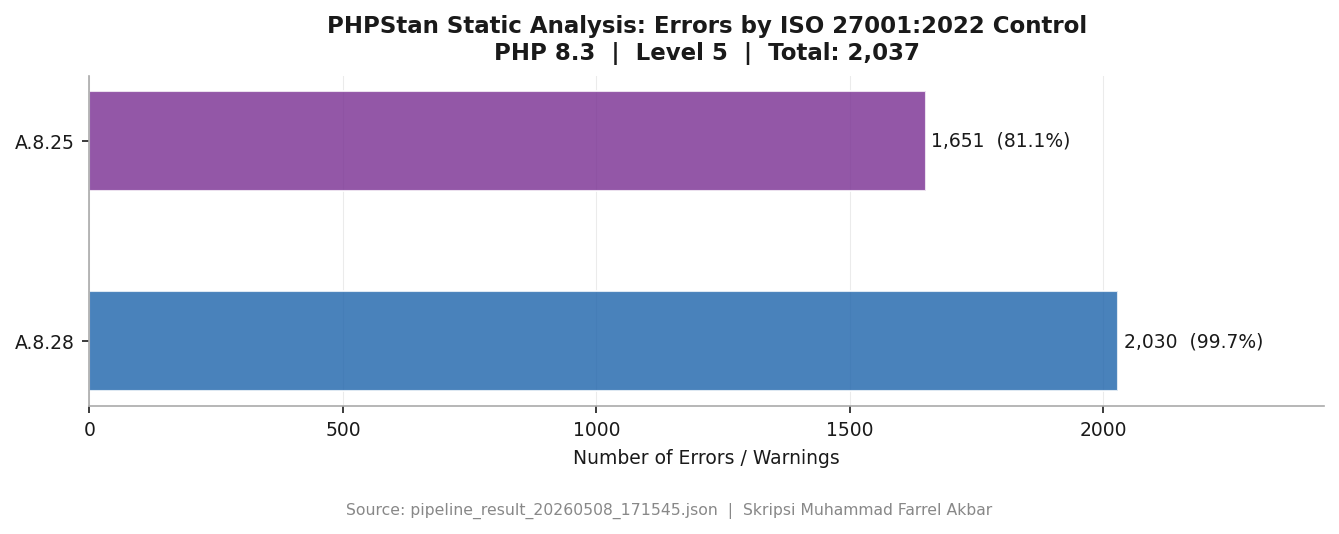
\includegraphics[width=1.0\textwidth]{contents/chapter-4/dti/pipeline_chart_20260509_074426_4_phpstan_iso.png}
    \caption{Distribusi temuan PHPStan berdasarkan kontrol ISO/IEC 27001:2022 Annex A pada dataset CBT DTI UGM}
    \label{fig:phpstan-iso-dti}
\end{figure}
\newpage
Sebagaimana pada studi kasus FT UGM, seluruh \textit{error} PHPStan pada 
dataset CBT DTI merupakan \textit{false positive} yang disebabkan oleh 
keterbatasan PHPStan dalam memahami arsitektur CodeIgniter 3.x. PHPStan 
tidak dapat menelusuri dua kategori elemen yang diinjeksi secara dinamis 
oleh \textit{framework} pada saat \textit{runtime}. Pertama, 
\textit{magic property}: yaitu properti kelas yang tidak dideklarasikan 
secara eksplisit dalam kode sumber melainkan diinjeksi melalui metode 
\texttt{\_\_get()} PHP seperti \texttt{\$this->db} dan 
\texttt{\$this->load} yang berasal dari \texttt{CI\_Controller} dan 
\texttt{CI\_Model}. Kedua, fungsi-fungsi \textit{helper} seperti 
\texttt{base\_url()}, \texttt{redirect()}, dan \texttt{form\_open()} yang 
dimuat secara dinamis melalui \texttt{\$this->load->helper()}. Karena 
direktori \texttt{system/} CodeIgniter dieksklusi dari analisis, PHPStan 
kehilangan definisi kelas induk dan fungsi-fungsi tersebut sehingga 
melaporkannya sebagai \textit{undefined}.

Pola distribusi \textit{error} PHPStan pada CBT DTI menunjukkan karakteristik 
yang berbeda dengan FT UGM: proporsi \textit{error} A.8.25 lebih tinggi 
(1.651 dari 2.037, atau 81,1\%) dibanding FT UGM (1.266 dari 2.871, atau 
44,1\%). Perbedaan ini mencerminkan komposisi kode yang berbeda: CBT DTI lebih 
banyak mengandung pola penggunaan \textit{magic property} CI3 yang memicu 
\textit{error} kategori \textit{Secure Development Lifecycle}, sementara FT UGM 
memiliki lebih banyak \textit{error} tipe dan kompatibilitas yang terdistribusi 
di kategori A.8.28.

% ------------------------------------------------------------
\subsection{Status Kepatuhan ISO/IEC 27001:2022}
% ------------------------------------------------------------

Berdasarkan pemetaan yang dilakukan oleh \texttt{iso\_mapper.py}, status 
kepatuhan terhadap enam kontrol ISO/IEC 27001:2022 yang dipetakan adalah 
sebagaimana ditunjukkan pada Tabel \ref{tab:iso-status-dti}.

\begin{table}[h]
\centering
\caption{Status kepatuhan ISO/IEC 27001:2022 hasil \textit{pipeline} pada dataset CBT DTI UGM}
\label{tab:iso-status-dti}
\begin{tabularx}{\textwidth}{|l|l|X|l|}
\hline
\textbf{Kontrol} & \textbf{Judul} & \textbf{Dasar Penilaian} & \textbf{Status} \\
\hline
A.5.17 & \textit{Authentication Information} & Tidak ada temuan \textit{hardcoded credentials} & \texttt{COMPLIANT} \\
\hline
A.8.24 & \textit{Use of Cryptography} & Tidak ada temuan penggunaan \texttt{md5()}/\texttt{sha1()} untuk kata sandi & \texttt{COMPLIANT} \\
\hline
A.8.25 & \textit{Secure Development Lifecycle} & 1.651 temuan PHPStan (\textit{false positive} CI3) & \texttt{NON\_COMPLIANT} \\
\hline
A.8.26 & \textit{Application Security Requirements} & Tidak ada temuan SQL Injection dari Semgrep & \texttt{COMPLIANT} \\
\hline
A.8.28 & \textit{Secure Coding} & 2.030 dari 2.037 ERROR PHPStan (\textit{false positive} CI3) & \texttt{NON\_COMPLIANT} \\
\hline
A.8.29 & \textit{Security Testing in Development} & Pemindaian Semgrep dijalankan, tidak ada temuan terbuka & \texttt{COMPLIANT} \\
\hline
\end{tabularx}
\end{table}
\newpage
Status keseluruhan adalah \texttt{NON\_COMPLIANT} karena adanya temuan 
PHPStan pada A.8.25 dan A.8.28. Perlu dicatat bahwa perbedaan status 
dibanding FT UGM terdapat pada A.8.26 dan A.8.29: kedua kontrol ini 
berstatus \texttt{COMPLIANT} pada CBT DTI karena tidak ada temuan Semgrep 
aktif, sementara pada FT UGM keduanya berstatus \texttt{NON\_COMPLIANT} 
dan \texttt{PARTIAL} akibat adanya temuan SQL Injection dan SSRF.

% ------------------------------------------------------------
\subsection{Analisis Dependensi Composer}
% ------------------------------------------------------------

Aplikasi CBT DTI UGM tidak memiliki berkas \texttt{composer.json} pada 
tingkat aplikasi. Komponen pihak ketiga seperti \textit{library} TCPDF 
disertakan langsung sebagai direktori dalam repositori dan telah dieksklusi 
dari analisis \textit{pipeline}. Oleh karena itu, modul 
\texttt{composer\_analyzer.py} tidak menghasilkan keluaran untuk studi 
kasus ini dan langkah analisis dependensi dilewati secara otomatis.

% ============================================================
\section{Perbandingan Kedua Studi Kasus}
% ============================================================

Bagian ini membandingkan hasil implementasi \textit{pipeline} pada kedua 
studi kasus secara berdampingan untuk mengidentifikasi pola yang konsisten 
maupun perbedaan yang signifikan.

% ------------------------------------------------------------
\subsection{Perbandingan Temuan Keamanan Semgrep}
% ------------------------------------------------------------

Gambar \ref{fig:comparison-semgrep} menunjukkan perbandingan temuan Semgrep 
\textit{pre-scan} berdasarkan jenis kerentanan pada kedua dataset.

\begin{figure}[h]
    \centering
    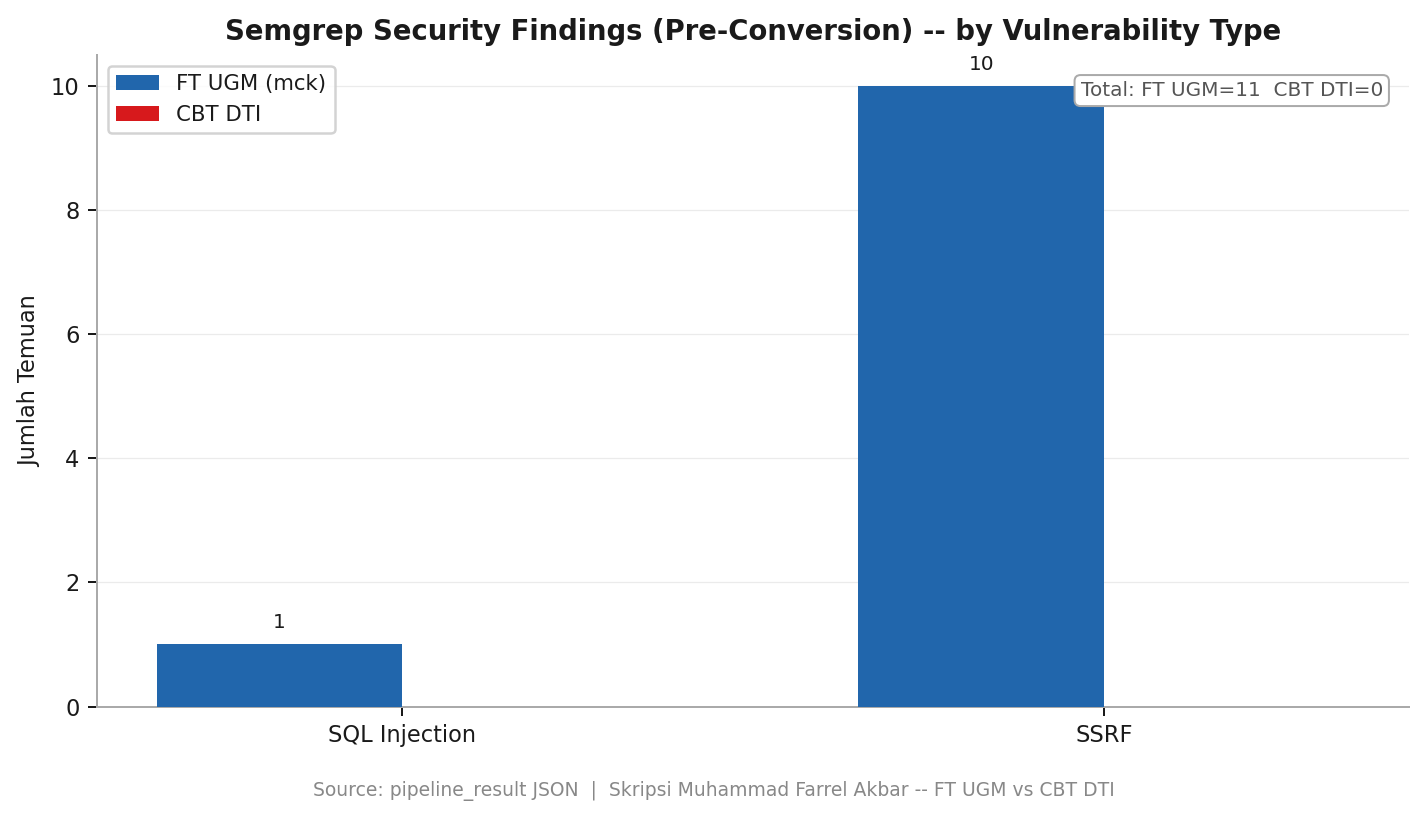
\includegraphics[width=0.95\textwidth]{contents/chapter-4/comparison/comparison_1_semgrep_findings.png}
    \caption{Perbandingan temuan Semgrep \textit{pre-scan} berdasarkan jenis kerentanan pada kedua studi kasus}
    \label{fig:comparison-semgrep}
\end{figure}

Dataset FT UGM mengandung 11 temuan aktif (1 SQL Injection dan 10 SSRF), 
sementara dataset CBT DTI tidak menghasilkan temuan sama sekali. Perbedaan 
ini tidak serta-merta berarti kode CBT DTI lebih aman secara absolut; 
melainkan mencerminkan perbedaan arsitektur dan cakupan kode yang dianalisis. 
Seluruh temuan FT UGM terpusat pada \texttt{Output.php}, sebuah modul 
\textit{framework} yang menangani operasi \textit{cache} dengan interaksi 
tinggi terhadap data eksternal. Modul setara pada CBT DTI kemungkinan 
berada di dalam direktori \textit{framework} yang dieksklusi dari pemindaian.
\newpage
% ------------------------------------------------------------
\subsection{Perbandingan Tingkat Konversi Rector}
% ------------------------------------------------------------

Gambar \ref{fig:comparison-rector} menunjukkan perbandingan hasil konversi 
Rector pada kedua dataset.

\begin{figure}[h]
    \centering
    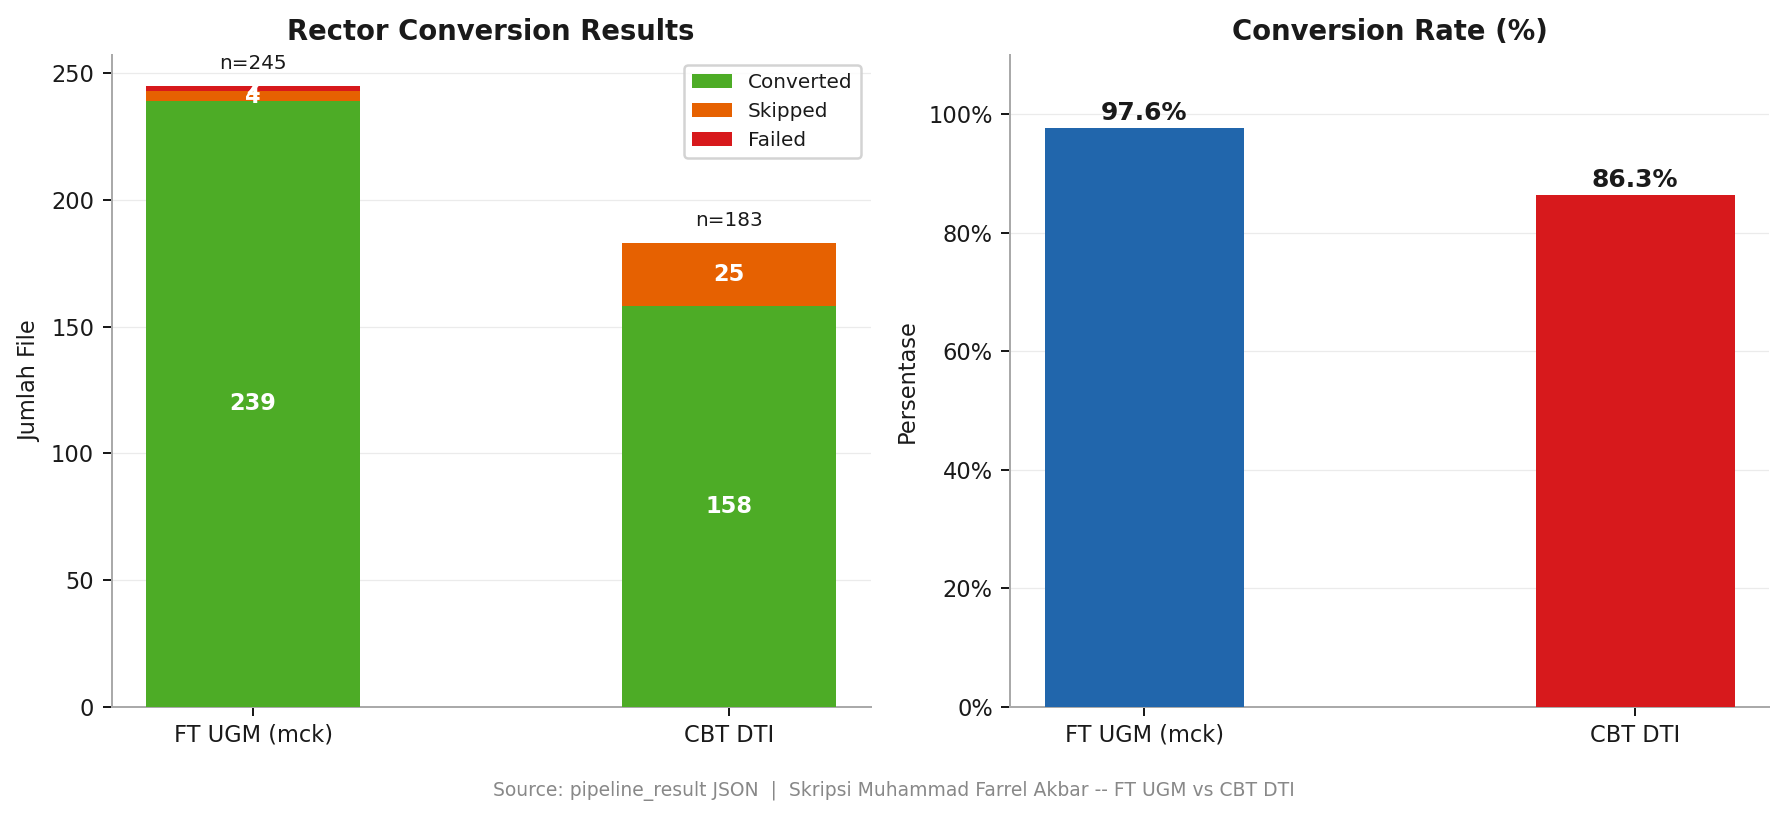
\includegraphics[width=0.98\textwidth]{contents/chapter-4/comparison/comparison_2_rector_conversion.png}
    \caption{Perbandingan hasil konversi Rector pada kedua studi kasus}
    \label{fig:comparison-rector}
\end{figure}
FT UGM mencatat \textit{conversion rate} 97,6\% (239/245) sementara CBT DTI 
mencatat 86,3\% (158/183). Perbedaan 11,3 poin persentase ini terutama 
disebabkan oleh proporsi \textit{file} yang dilewati: CBT DTI memiliki 
25 \textit{file} \textit{skipped} (13,7\%) dibanding 4 \textit{file} pada 
FT UGM (1,6\%). \textit{File} yang dilewati adalah \textit{file} yang sudah 
kompatibel dengan PHP 8.3 atau tidak mengandung pola yang perlu ditangani 
Rector, sehingga \textit{skipped} bukan berarti gagal melainkan sudah 
kompatibel dengan PHP 8.3. FT UGM juga memiliki 2 \textit{file} yang gagal diproses akibat 
\textit{bug} \texttt{FiberNodeScopeResolver}, sementara CBT DTI tidak 
mengalami kegagalan yang sama. Pada kedua studi kasus, validitas sintaks 
pasca-konversi mencapai 100\%.

% ------------------------------------------------------------
\subsection{Perbandingan Temuan PHPStan}
% ------------------------------------------------------------

Gambar \ref{fig:comparison-phpstan} menunjukkan perbandingan distribusi 
\textit{error} PHPStan berdasarkan kontrol ISO/IEC 27001:2022 pada kedua 
dataset.

\begin{figure}[h]
    \centering
    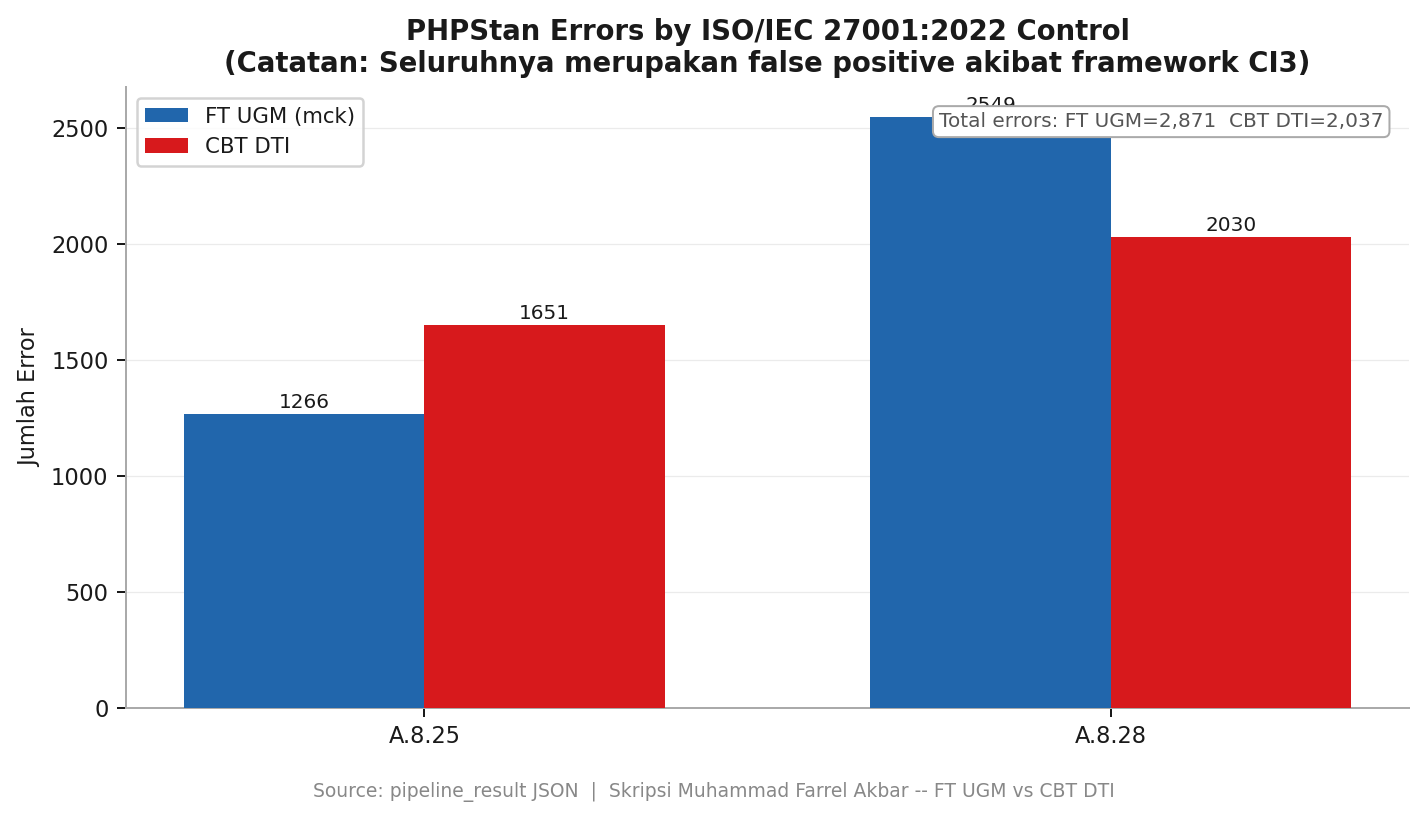
\includegraphics[width=0.98\textwidth]{contents/chapter-4/comparison/comparison_3_phpstan_iso.png}
    \caption{Perbandingan \textit{error} PHPStan berdasarkan kontrol ISO/IEC 27001:2022 pada kedua studi kasus}
    \label{fig:comparison-phpstan}
\end{figure}

FT UGM menghasilkan 2.871 \textit{error} PHPStan sementara CBT DTI 
menghasilkan 2.037 \textit{error}. Keduanya dijalankan pada PHPStan 
\textit{level} 5 dengan target PHP 8.3, sehingga angka ini dapat 
dibandingkan secara langsung. Seluruh \textit{error} pada kedua dataset 
merupakan \textit{false positive} akibat keterbatasan PHPStan terhadap 
arsitektur CodeIgniter 3.x sebagaimana dijelaskan pada subbab sebelumnya. 
Jumlah \textit{error} yang lebih tinggi pada FT UGM sebanding dengan 
ukuran dataset yang lebih besar (245 vs 183 \textit{file}) dan penggunaan 
dependensi pihak ketiga yang lebih beragam.

% ------------------------------------------------------------
\subsection{Ringkasan Perbandingan dan Analisis Dependensi Composer}
% ------------------------------------------------------------

Gambar \ref{fig:comparison-summary} merangkum seluruh metrik utama kedua 
studi kasus dalam satu tampilan, termasuk status dependensi \textit{composer} 
FT UGM.
\begin{figure}[h]
    \centering
    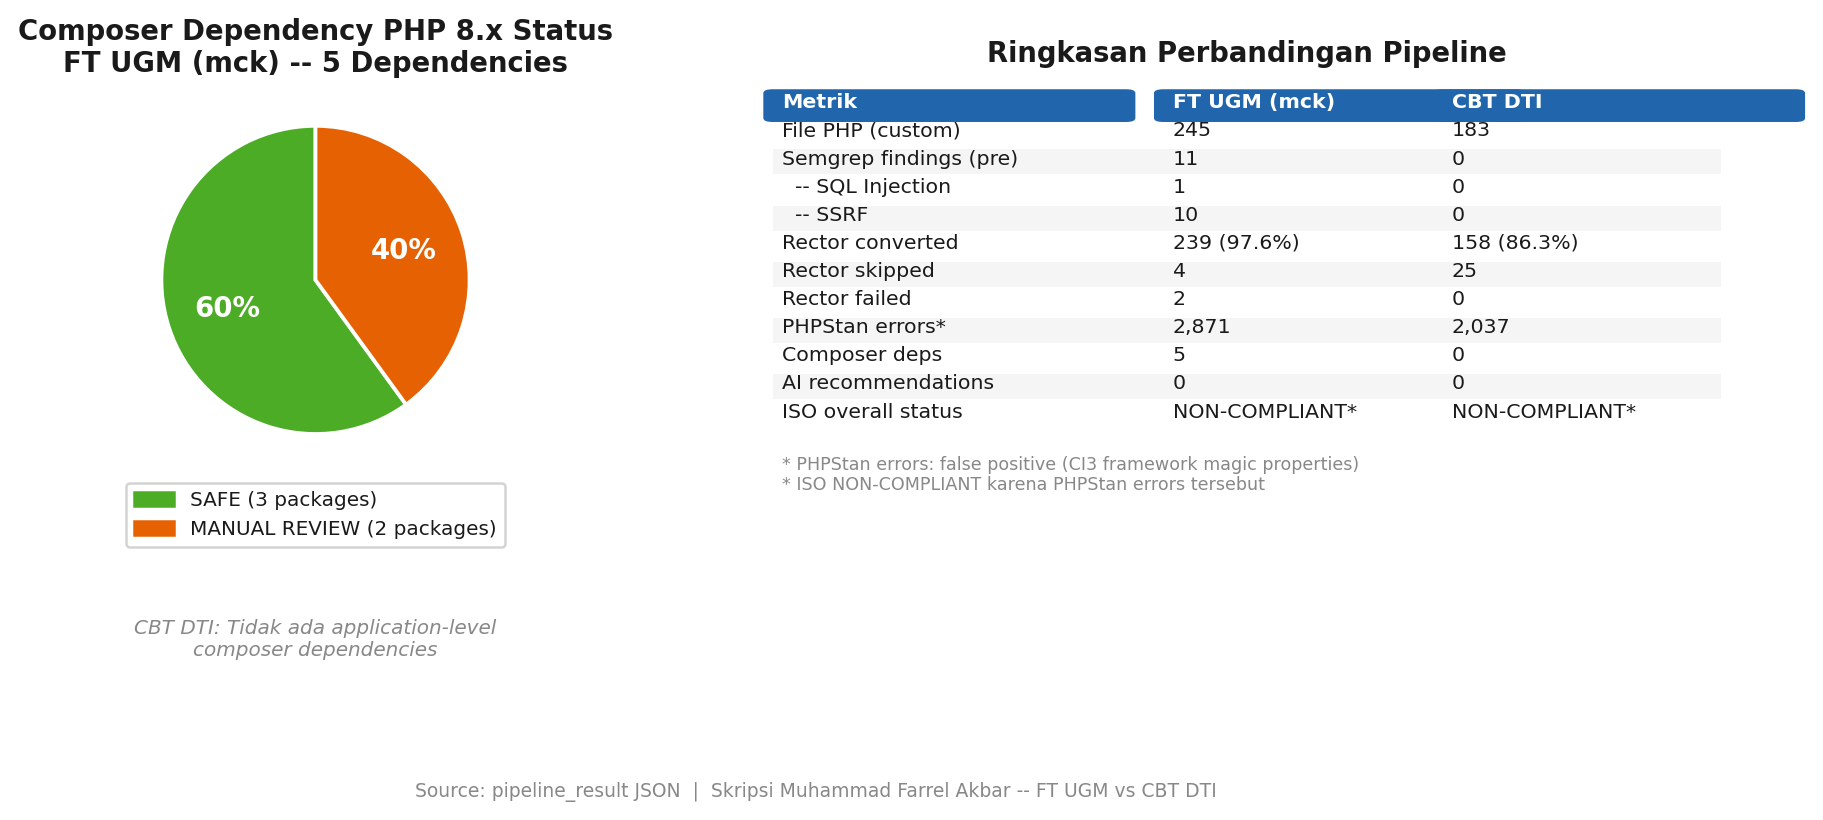
\includegraphics[width=\textwidth]{contents/chapter-4/comparison/comparison_4_composer_summary.png}
    \caption{Ringkasan perbandingan metrik \textit{pipeline} dan status dependensi \textit{composer} kedua studi kasus}
    \label{fig:comparison-summary}
\end{figure}

Secara keseluruhan, kedua studi kasus menunjukkan pola yang konsisten: 
\textit{pipeline} berhasil menjalankan seluruh tahapan secara otomatis, 
konversi Rector menghasilkan kode yang valid secara sintaksis di kedua 
dataset, dan status ISO/IEC 27001:2022 keduanya adalah \texttt{NON\_COMPLIANT} 
yang disebabkan oleh \textit{error} PHPStan. Perbedaan utama terletak pada 
keberadaan temuan Semgrep: FT UGM memiliki kerentanan aktif yang memerlukan 
remediasi manual, sementara CBT DTI bersih dari temuan Semgrep pada kode 
kustomnya. Perbedaan lain adalah durasi eksekusi: FT UGM membutuhkan sekitar 41 menit karena eksperimen LLM 
dijalankan terhadap 11 temuan Semgrep, sementara CBT DTI selesai 
dalam sekitar 50 detik karena langkah AI Engine dilewati akibat 
tidak adanya temuan Semgrep.
